\documentclass[12pt]{article}

\usepackage{amsmath}
\usepackage{graphicx}
\usepackage{tabularx}
\usepackage{natbib}
\usepackage{todonotes}
\usepackage{amssymb}
\usepackage{amsfonts}
\usepackage{amsthm}
\usepackage{mdframed}
\usepackage{float}
\usepackage[labelfont=bf]{caption}
% To do commands
\newcommand{\slava}[1]{\todo[color=blue!40]{#1}}
\newcommand{\trish}[1]{\todo[color=green!20]{#1}}

\linespread{1.6}

\title{Master's Proposal}
\author{Slava Nikitin}
\date{\today}

\begin{document}
\maketitle

\tableofcontents

\trish{
%%%%%%%%%%%%%%%%%
Things to do:
\begin{itemize}
\item Correct all noted errors.  I expect your revision to begin on
      this version of the document, and not from a version of your own with
      my changes copied into it.  I may have made small corrections along
      the way without flagging them, and I have no intention of doing them a
      second time.
\item List/Describe/Explain the features of the data explained by the
      Ratcliff diffusion model and how the model accomplishes these things.
      E.g., fast and slow errors and what allows the model to produce them.
\item Make a better case that we need to model parameter covariance over 
      trials.  Find outside references to support your case.
\item Rewrite your presentation of copulas using a specific example.
      E.g.: Here is a bunch of exponential marginals with correlated
      parameters (write down the distributions).  Then hereis the copula
      (write down $C$).  Etc.
\item Rewrite your description of MCMC methods so that it can be
      understood by someone who has never heard of them before.
\item Use the "algorithm" package for the figures containing pseudocode.
\item Section 3.4 must be completely rewritten.  It is "nonlinear,"
      and incomprehensible to a naive reader.  Take is apart, and use
      subsections to describe the subcomponents of the sampler.  Define all
      terms and describe all examples from the ground up.
\item Quite late in the document you write that Ratcliff's mixture
      model is in some way equivalent to a Bayes model where the mixture
      probabilities play the role of priors.  This is not true (see my note
      at that point).  You must expand your description of the model and
      organize the presentation of its components so that either this
      confusion is eliminated or so that it is clear that you are not in
      fact presenting a Bayesian treatment of the Ratcliff model.

\item The Ratcliff/Rouder study should be presented first, before your
      Studies.  Use the RatRou experiment to motivate the other
      sections of the proposal, when you need an example to refer to
      (see notes throughout).
\item Eliminate the portion of your proposal that models outliers.
      This means that you need to rewrite Study~C as something much more
      modest.  See my comments there.
\item Restructure the proposal in chapter format: 
\begin{itemize}
      \item Introduction (including Literature Review and discussion
      of Bayesian Methods).  I think you need at least four sections
      here: The diffusion model, a discussion of copulas with worked
      out example, Bayesian methods, and the RatRou study.
      \item Statement of the Problem or Proposed Work.  Include here
      an outline explaining exactly what you are going to do as it is
      presented in your proposal.  Your current Section 2 bears little
      resemblance to what you propose to do as it is laid out in later
      sections.
      \item Modeling.  Include here the diffusion model, how the
      parameters will be modeled, how copulas will be incorporated,
      etc.
      \item Studies.
      \item See the next item.
\end{itemize}
\item Add segues.  Every transition at every level (sentences,
      paragraphs, sections) requires a segue.  Read your writing
      carefully, with an eye for abrupt "jumps" between ideas.
      Remember the general rule of a talk should be followed in a
      paper: Tell people what you're going to tell them, tell them
      that, then tell them what you just told them. 
\item Add your reference section.  In the future, please consider the
      reference section a required portion of any written document, even
      rough drafts.  
\end{itemize}

%%%%%%%%%%%%%%%%%%%%%%%%%%%%%%%%%%%%%%%%%%%%%%%%%%%%%%%
\section{Introduction}

The basic fact that underpins this proposal is that every statistical model
\trish{of a cognitive process} is a simplification \trish{and therefore}
limited in \trish{the} inferences it supports. If \trish{the} questions
motivating research go beyond the inferential capacity of a model, then it
is natural to construct a new one. The \trish{problem I address in this
proposal} is whether and in what way \trish{the} psychological processes
responsible for simple decision making are coordinated across trials to
perform two-choice tasks (e.g., does the stimulus move right or
left?). \trish{My explorations of this problem} will enrich understanding
of sequential properties of cognitive processing.

A long history of investigating simple decisions points to \trish{the time
to encode} stimulus features, rate of information uptake, level of caution,
decision bias and \trish{time to execute a} response as key psychological
parameters driving performance
 \citep{Sto1960,Vic1979,TowAsh1983,Luc1986,BogRaf2006}.  

\trish{Comment:
 The remainder of this paragraph is hard to understand.  What are you
 trying to say?  We already know that there is a speed-accuracy tradeoff
 across blocks of trials or experimental conditions.
 Are you trying to say something about controlling a SA tradeoff on a
 trial-by-trial basis?  If so, what is the evidence that such a thing might
 exist, or what data point to such a thing?}  

\trish{{\em{previous paragraph cont.}} Evidence for} 
coordinated adjustments of psychological processes would be present if
sensible tradeoffs between parameters took place to maintain a
\trish{balance between, for example, speed and accuracy.  If} all key
processes are involved in controlling the \trish{balance} between speed and
accuracy, then to raise accuracy a sensibly-designed cognitive system would
\trish{require an} increase {\trish{in the} time for stimulus processing,
rate of information uptake, level of caution, \trish{NO: delete remove
decision bias} and response execution time. \trish{Similarly, to increase
speed, the system would require that all these parameters be reduced.
Therefore the} presence of \trish{trial-by-trial} tradeoffs \trish{must
result in} statistical dependencies among parameters \trish{estimated
across trials}.

However, in \trish{most} applications of prominent models of simple
decisions, it is common to assume that psychological parameters fluctuate
across trials in a mutually independent manner
\citep{RatTue2002,UshMcc2001,BroHea2008}. The implication of the
independence assumption is that there is no general, long-term coordination
of processes. Instead, processes could be adjusted \trish{delete:
arbitrarily} through selective experimental manipulations
\citep{VosAnd2004}. For example, giving instructions to participants to
emphasize speed or accuracy \trish{is usually assumed to} affect only the
caution parameter
\citep{RatMck2008,Wag2009,VanTue2007,VanTue2011,RaeHea2014}. Change in
caution would not correlate with any other parameter.
    
\trish{I don't understand this paragraph. How could lack of coordination be
consistent with coordination?  What does it mean to stretch a sequence?
You seem to imply that post-error slowing is a one-shot deal, and not the
result of the seuence of trials that came before the error.  Do you have
evidence that this is the case?  You cite evidence against this position
late in the paragraph.  Rewrite.}  Also, the lack of general coordination
is also consistent with coordinated adjustment, stretching short sequences
of trials. In this case, different sequences would have different tradeoffs
leading to long run independence. For example, post error slowing is a
short-term phenomenon that arises from participants monitoring their
performance and adjusting their processing to maintain a relatively
constant level of accuracy \citep{VanMal2004}. While a common suggestion is
that slowing is solely due to caution increase, a recent study comparing
old and young adults showed evidence for coordinated changes
\citep{DutFor2013}. Model-based analysis concluded that rate of uptake
decreased, caution increased and nondecision time increased. However, the
post error pattern of parameter adjustments may not represent a general
trend of coordination, and change over the next few trials.
    
While both selective influence of processes and short-term dependencies of
post error slowing support the notion that \trish{You haven't made the case
for this: there is no general coordination of cognitive processes}, I would
like to test it more directly. \trish{Delete: A common approach to
answering questions about cognitive processing is to build a mathematical
model. Statistically, dependencies imply associations among parameters that
are assumed to vary across trials. (You've already said all this above.)}
The dominant class of cognitive process models developed to account for
simple decision making lacks \trish{a formal} structure to make inferences
about process dependencies \citep{SmiRat2004} \trish{(Do they say this, or
is this your reference for the dominant class?). Thus, \trish{one purpose
of my thesis is to modify these statistical models to provide a structure that can
incorporate and permit measuring the extent of parameter dependence}.
    
\trish{Specifically,} I propose to take an empirically well-tested model of
simple decisions and add an association structure that shapes how
parameters fluctuate across trials. The model will enable testing the
assumption of independent parameters that implies no general coordination
of processes and measuring whatever associations that could be present.
    
The proposal will unfold in the following way. First, I discuss why the
cognitive process model is \trish{the} approach I take to answer the
question about process coordination and dependencies. Then, to provide
context, I will introduce \trish{Huh?: the simple decision making
phenomenon} and discuss how it is studied in the laboratory. Third, I will
introduce \trish{the} sequential sampling framework for modeling simple
decisions, and focus on the Ratcliff diffusion model, a prominent
sequential sampling model that can account for \trish{the} main features of
experimental data. Fourth, I will describe specific problems in developing
models with association structure and \trish{present a} methodology for
solving them. Finally, I will \trish{propose} three studies that should
provide answers to the posed problems.

%%%%%%%%%%%%%%%%%%%%%%%%%%%%%%%%%%%%%%%%%%%%%%%%%%%%%%%
\subsection{Development of Cognitive Models}

\trish{Much better!}
Psychology has as one of its chief aims identification of the cognitive
architecture that generates the rich repertoire of human behavior and is
sensitive to many environmental variables \citep{AndBot2004,And2007}. More
specifically, a psychologist wants to learn about the number, temporal
arrangement, individual characteristics and interactions of elementary
processes and \trish{representations of what?}. A fundamental obstacle is
that cognition is not directly observable. From the perspective of systems
identification, the study of human cognition is an instance of a black box
problem \citep{Lju1999, Lju2010}. Working on a black box problem, a
researcher only has direct information about the system's input and
output, but lacks direct access to internal processes transforming inputs
into outputs. The problem then is how to identify internal processes from
known combinations of inputs and outputs, that is, how to uncover the human
cognitive architecture from information about overt behavior taking place
in some environment.

An approach to providing an approximate solution to the black box problem
is \trish{the} construction of competing mathematical models that can be
tested against data using statistical methods
\citep{Lju1999,Lju2010,CasBer2002,GelCar2013}. A model that best balances
parsimony, fit to empirical regularities and interpretability can be taken
as an approximate solution \trish{to what?}, and provide valuable insights
about internal processes. This approach fits well with psychological
phenomena because it is often easy to come up with several, categorically
different conjectures about the underlying cognitive processing
\citep{TowAsh1983}. \trish{You already said this in the first sentence,
delete or rewrite: The best way to ensure coherency of conjectures about
cognition \trish{nice alliteration!}, and improve their falsifiability, is
to formalize them in mathematical models
\citep{BusDie2010,LewFar2010,LeeWag2014}.} For instance, a model that can
predict a power relation between time and memory retention is easier to
falsify than a verbal account that only makes ordinal predictions
\citep{CavMyu2013}. Ultimately, the goal is to use models of cognition to
draw insights about elementary processes and how they change under
experimental manipulations, across individuals and \trish{across} groups.


\trish{Made small punctuation changes in here.  Note that I prefer you to
reserve the use of quotation marks for responses and for first-time
definitions.  Don't continue to use quotation marks for things you have
already defined.  If you want, you could use italics or some other font
face to set off the stimulus classes, but only ``yes'' and ``no'' should be
in quotes.  Note also smart quotes, which take `` at the beginning and ''
at the end.  Your quotes are garbled, which happens sometimes depending on
the word-processor you are using.  Because of this problem I tend to type
them in by hand:} A paradigm case of modeling cognition is signal detection
theory \citep{MacCre2004}. The original phenomenon motivating development
of signal detection models was human ability to make decisions with
distorted sensory stimuli. This phenomenon can be studied experimentally
using a computerized task. For example, during the auditory signal
detection task an observer is presented with a sequence of stimuli drawn
either from a ``Signal'' distribution representing a tone combined with
white noise, or a ``Noise'' distribution representing white noise. On each
trial, an observer has to respond ``Yes'' if he \trish{or she} decides the
stimulus belongs to the Signal distribution and ``No'' otherwise. Under
these conditions, a researcher knows which class each presented stimulus
belongs to and observes a sequences of responses, typically summarized as
hit rate (proportion of true positive \trish{responses}) and false alarm
rate (proportion of false positive \trish{responses}). The problem is to
learn about cognitive processes involved in transforming stimulus
information into responses from the generated data.

\trish{Careful here.  People will argue with you about this
characterization.  Is SDT a theory of how decisions are made or is it a
model of simple choice?  Many people, myself included, would say that SDT
does not make any claims about the cognitive processes underlying the
decision.}  Signal detection models are probabilistic models that specify
how elementary cognitive processes operate on information contained in
external stimulus to produce hits and false alarms
\citep{MacCre2004,LeeWag2014}. The basic idea is that \trish{behavior in a}
signal detection \trish{task} can be \trish{explained by a theory that
proposes the following:}
%
\trish{This is more a set of instructions to simulate performance of a SD
task than a theory.  I have commented out what I perceive to be
non-cognitive processes and changed what remains:}
%
\begin{enumerate} 
% \item Sample randomly a stimulus from either a Signal or Noise class 
% \item Sample randomly a strength value given a class of the stimulus 
% \item If the strength value is greater than or equal to a threshold then 
%       respond ``Yes,'' otherwise respond ``No.''  
% \item Repeat steps $1$--$3$ for N trials 
%
\item Presentation of a stimulus leads to an observer's perception of
      stimulus ``strength.''  
\item An observer is able to establish a threshold to which this perceived 
      strength can be compared.  
\item If the perceived strength is greater than this threshold then the 
      observer responds ``Yes,'' otherwise he or she responds ``No.''  
\item The perceived strength is a random variable whose behavior (mean and 
      variance) is determined by the class of the presented stimulus, such 
      that the strengths of Noise stimuli tend to be perceived as being below 
      the threshold and the strengths of Signal stimuli tend to be perceived 
      as being above.  
\end{enumerate} 
\trish{Note that if you put a blank line in latex, that tells it to break
to a new paragraph.  It means that everything following the blank line
should be indented, etc.  If you want blank lines for ease of reading or
typing, start them with a %.}

Mathematically, let a random variable $C \in \{0, 1\}$ represent a stimulus
randomly drawn either from \trish{the} Noise class \trish{($C=0$)} or
\trish{the} Signal class \trish{($C=1$)}. The probability mass function of
$C$ is determined by the experimenter. In response to the sampled
\trish{stimulus,} an internal representation of strength value, represented
by a random variable $X \in \mathbb{R}$, is generated. \trish{We commonly
assume that} $X$ conditioned on \trish{the} stimulus class is normally
distributed with class-specific mean and variance \trish{parameters, so that}
%
\begin{align}\nonumber
X \mid C = 1 \sim \mathcal{N}(\mu_s, \sigma_s^2) \trish{\text{ and } \\
X \mid C = 0 \sim \mathcal{N}(\mu_n, \sigma_n^2)\trish{.}
\end{align}
%

\trish{Problem here.  Tau can't be the distance from the midpoint and be
the threshold.  Either the threshold is $\tau$, in which case it is a
location, or it is $c-\tau$ for $\tau \in \mathbb{R}$.  You choose, but as
written this is wrong.}  Finally, let $\tau$ represent a threshold which is
defined as the distance from a point ${\trish{c=}\frac{\mu_s \trish{+}
\mu_n}{2}}$, \trish{which is the midpoint between the means of the Signal
and Noise distributions.  If the distributions have common variance
$(\sigma_s = \sigma_n)$, then $c$ is the location where the two probability
density functions intersect.}  Then a random variable
%
\trish{Small changes below:}
\begin{equation}
R = \left\{
	\begin{array}{l l}
     1 & \text{ if } X \geq \tau\\
     0 & \text{ if } X < \tau
     \end{array}\right.
\end{equation}
%
represents a ``Yes'' ($R=1$) or \trish{a} ``No'' ($R=0$) response.
\trish{Note that "respectively" is only used when lists follow lists and
not when lists follow equations.}

% You might like to read Halmos (1970), "How to Write Mathematics."

\trish{Note: Below you switch to $d'$ and $\tau$, so make sure you state
that you are talking about "derived" parameters here.  Again, for SDT, I
would strongly advise you to avoid making claims about cognitive
processes.}  \trish{As written, this} version of the model has five free
parameters \trish{($\mu_n,\mu_s,\sigma_n,\sigma_s,\tau$)}, but
\trish{because normal distributions form a location-scale family, where the
mean and standard deviation are the location and scale parameters,
repectively, the means and standard deviations are identifiable only
relative to each other.  Therefore, we set} $\mu_n = 0$ and $\sigma_n = 1$
\trish{without loss of generality}. The other three parameters remain free
and quantify central features of processing supporting signal detection.
%
\trish{No, $d'$ depends on $\sigma_s$.  If you are assuming that
$\sigma_s=1$ then say so, but I don't think that's what you intend:}  The
sensitivity parameter, $d' = \mu_s - \mu_n = \mu_s$, quantifies how well
the encoding process separates Noise from Signal stimuli. 
%
\trish{Remember that you need to fix this.  Seems to me that $\tau$
measures bias as you've defined it, not the threshold:} The threshold
$\tau$ represents the decision criterion
%
and the ratio of variances
$\frac{\sigma_n^2}{\sigma_s^2} = \frac{1}{\sigma_s^2}$ between Noise
and Signal distributions characterizes relative noise in
representations. These three parameters drive the predicted pattern of
responses.
    
To begin testing a specified cognitive model one needs to derive, or be
able to simulate, predictions for performance data. In the signal detection
case, the random mechanism specified above, and an additional assumption
that all responses during an experiment are mutually independent, allow for
an analytical derivation of a probability mass function parameterized by
the three free parameters.  The derived model for \trish{the number of hits
$Y_h \in \{0, 1, \ldots, N_s\}$ and the number of false alarms $Y_{fa} \in
\{0, 1, \ldots, N_n\}$} for a given participant \trish{presented with $N_s$
Signal stimuli and $N_n$ Noise stimuli} is a product of two binomial mass
functions.  \trish{The joint probability of $Y_h=y_h$ and $Y_n=y_n$ is therefore}
%
\trish{Formatting changes:
\begin{eqnarray}
\lefteqn{f(y_h, y_{fa} \mid p_h, p_{fa}, N_s, N_n) = }\nonumber \\
\binom{N_s}{y_h}p_h^{y_h}(1 - p_{h})^{N_s - y_h}
\binom{N_n}{y_{fa}}p_{fa}^{y_{fa}}(1 - p_{fa})^{N_n - y_{fa}}
\end{eqnarray}
}
%
with \trish{the probabilities $p_h$ and p_{fa}$ being the probabilities
that $R=1$ conditioned on the stimulus class.  These probabilities are in
turn functions of the parameters $d'$, $\tau$ and $\sigma_s$, so 
%
\begin{align}\nonumber
p_h = P(R = 1 \mid C = 1) = \Phi(\frac{0.5d' + \tau}{\sigma_s}) \text{ and } \nonumber \\
p_{fa} = P(R = 1 \mid C = 0) = \Phi(-0.5d' - \tau),
\end{align}
where $\Phi( )$ is \trish{the standard} normal cumulative distribution function.
    
\trish{When} a statistical model relating cognitive parameters \trish{to}
data is specified for a given theory, one can use a rich body of
statistical methods to explore its predictions via simulations, to estimate
its free parameters from data, \trish{and} to compare and select from
competing models of a cognitive processing involved in a given task
\citep{Ber1997,CasBer2002,GelCar2013}. Connecting the signal detection
model to performance data enables a researcher to make a range of
inferences about cognitive processes involved in signal detection. For
instance, it is possible to test goodness of fit of a model with
$\sigma_s^2 = 1$ against a model where $\sigma_s^2$ is a free parameter to
determine \trish{the} noise properties of \trish{the} stimulus
representation. However, the range of possible inferences is limited, so
the specified model cannot say anything about \trish{(for example)}
adaptations of the representations \trish{to what?} or motor processing. It
would require a new model to address additional questions about signal
detection.


%%%%%%%%%%%%%%%%%%%%%%%%%%%%%%%%%%%%%%%%%%%%%%%%%%%%%%%
\subsection{\trish{wrong word: Phenomenon} of Simple Decision Making}

Developing new cognitive process models is a central tool for learning
about \trish{delete: the} human cognitive architecture
\citep{BusDie2010,LewFar2010,LeeWag2014}. The main problem addressed in
this thesis is a generalization of a well-established cognitive process
model of simple decision making in a way that enriches potential insights
about process interactions drawn from behavioral data. Before discussing
models, I will briefly delineate the simple decision making problem
motivating models of interest, and discuss experimental designs used to
\trish{determine} empirical regularities against which the models can be tested.
    
The psychological problem of interest can be posed in this way: how does a
human observer, in a short amount of time and with above chance accuracy,
choose, according to a preset rule, among a discrete set of responses using
confusable sensory stimuli? Computationally, the problem is to map stimulus
information into action \citep{Vic1979,BogRaf2006}. A variety of tasks
could be constructed to study \trish{the} underlying processes by varying
the sensory modality, the number of choices, the number of stimulus
attributes relevant to the decision, response modality and whether a
participant or an experimenter controls decision timing. I will concentrate
on participant-controlled \trish{timing?} two-choice tasks, driven by a
single \trish{attribute} of a stimulus. These tasks have been extensively
used in experiments and for developing cognitive models of simple decision
making, thus they make a solid starting point for \trish{developing a new
model (you aren't developing a new model, you're generalizing an old one.
Are you talking about what you're doing or what others have done?}
\citep{Luc1986,RatSmi2004,RatMck2008,Wag2009}.
    
An example of a two-choice task is a \trish{numerosity} task \citep{RatLov2012}. On
a given trial, two clouds of points consisting anywhere from a few dots to
hundreds are presented simultaneously. The relative number of dots is
deliberately picked to be similar to induce uncertainty about the correct
decision, and create imperfect performance. An observer has to make a
decision according to a rule such as ``pick the cloud with the larger
number of points'' within a short period of time, ranging roughly from 250
to 1000 milliseconds \citep{RatLov2012}.
    
Other two-choice paradigms include deciding in which direction dots are
moving, deciding whether a distorted character is an English letter,
deciding which pixelated square is brighter, and deciding whether a word
was studied before or not
\citep{SmiRat2004,RatSmi2004,RatRou1998,PerVan2002}. The data generated by
these tasks often include response times and responses under a variety of
\trish{delete: robust} experimental manipulations \citep{Luc1986}. For example, when
deciding whether a distorted character is an English letter a researcher
could vary level of distortion, probabilities of English and non-English
letters, and instructions emphasizing either speed or accuracy in
decisions. \trish{which? Empirical patterns} arising from these manipulations can be
repeatedly detected in response time distributions for correct and error
responses, response proportions, and relations between response proportions
and corresponding mean response times. In total, two-choice tasks tap into
a relatively tractable psychological problem, and provide a rich empirical
record to test abstract cognitive process models.
    
%%%%%%%%%%%%%%%%%%%%%%%%%%%%%%%%%%%%%%%%%%%%%%%%%%%%%%%%%%%%%%%%%
\subsection{Sequential Sampling Models}

A common approach to modeling cognitive processing underlying two-choice
tasks is to decompose \trish{them} into processes of encoding of stimulus
features, response selection based on a relevant stimulus feature and motor
execution. A cognitive process model for these tasks should make sufficient
assumptions about these processes to predict patterns in performance
data. A delicate balance has to be struck between what details to include
and what details to exclude \trish{from what? What details?} because it
will determine generalizability of models across two-choice tasks. For
instance, including details about how lexical information is accessed in
memory to direct response selection will make a model inapplicable to
brightness discrimination. The dominant approach to this balancing problem
is sequential sampling \trish{models}.
    
A fundamental theoretical assumption of sequential sampling \trish{models}
is that the same general decision process operates across all two-choice
tasks. Then, a generalizable model should provide a detailed account of the
decision process while making few assumptions about the stimulus encoding
and motor processing. Over the last $~50$ years, many models of this type
have been developed, and some of \trish{the} most successful \trish{ones}
can explain all the major patterns in the response time and response data,
under a variety of experimental conditions and tasks
\citep{Sto1960,Rat1978,RatTue2002,Smi1995,UshMcc2001,BroHea2008}. Some
models have also been used for predicting firing rates in neural
populations representing choices
\citep{RatChe2003,RatHas2011,SmiRat2004,Bog2007}, but I will concentrate on
performance data.
    
The underlying principle of sequential sampling models is that when an
observer is tasked with selecting the correct response, in limited time
\trish{from a} noisy stimulus, he \trish{or she} samples and integrates
information from the relevant stimulus \trish{attribute} until one of two
decision thresholds is reached
\citep{Sto1960,Edw1965,Pik1973,Rat1978,UshMcc2001,RatSmi2004,SmiRat2004,
RatMck2008,Wag2009,Luc1986,TowAsh1983,BogRaf2006}. By controlling
\trish{these} thresholds, the observer can balance the trade-off between
speed and accuracy of \trish{responses} \citep{BogWag2010}. \trish{What
does this mean: Bounded accumulation?} of information naturally provides
\trish{which? predictions of performance data} collected during two-choice
tasks. Accumulation times vary from run to run to produce distributions of
response \trish{times} and which threshold is reached first determines the
response.
    
Given the sequential sampling principle, any concrete model of simple
decisions makes detailed assumptions about the nature of sampled
information, temporal structure of sampling, stopping rule and sources of
randomness \citep{RatSmi2004,BogRaf2006,TeoUsh2013}. Combinations of
modeling assumptions generate the range of possible sequential sampling
models. For example, the sampled information can consist of discrete or
continuous packets. The size of the packets may be fixed or variable. The
accumulation of information packets may happen at fixed or variable
discrete time points, or continuously. The stopping rule may be absolute,
in which case accumulation stops when evidence in favor of one of the
choices reaches a threshold, regardless of the amount of evidence favoring
the alternative. In contrast, the relative rule requires that evidence
favoring one of the choices has to exceed the other by some amount.
    
Examples of sequential sampling models include a random walk model that
stops accumulation of discrete packets of randomly varying information over
discrete time according to a relative rule \citep{Lam1968}, a Poisson
counter model that continuously accumulates discrete, fixed information
packets until evidence for either of the choices reaches a threshold
\citep{Lab1962}, and a Wiener diffusion model that describes accumulation
of continuous packets in continuous time until a relative threshold
\citep{Rat1978}. I will concentrate on an empirically successful Ratcliff
diffusion model \citep{RatTue2002} as a base for incorporating assumptions
about process associations.
    
%%%%%%%%%%%%%%%%%%%%%%%%%%%%%%%%%%%%%%%%%%%%%%%%%%%%%%%%%%%%%%%%%
\subsection{Ratcliff Diffusion Model}

The Ratcliff diffusion model is a variant of the Wiener diffusion model
\trish{use bibtex cites consistently to avoid mistakes as references are
added and deleted during editing: (Laming, 1968; Link and Heath, 1975;
Ratcliff 1978; Ratcliff and Rouder, 1998; Ratcliff and Tuerlinckx 2002)}. I
concentrate on this model because of its long development \trish{delete:
and examination} (Ratcliff, 1978; Ratcliff and Rouder, 1998; Ratcliff,
2002; Ratcliff and Tuerlinckx, 2002; Ratcliff, 2013), and successful
testing against a wide range of experimental data (Ratcliff and McKoon,
2008; Wagenmakers, 2009). As with all sequential sampling models,
predictions about performance data are primarily implications of the
structure of the information integration process formalized in the language
of stochastic processes (Ross 2014; Karlin and Taylor, 1975, 1981).
    
Underlying the Ratcliff model is a continuous time, continuous state space
stochastic process that begins at some starting point and evolves until
\trish{it reaches} one of two absorbing boundaries. Formally, it is an
uncountable, ordered collection of univariate random variables 
%
\begin{equation} 
\{X(t); t \geq 0\} 
\end{equation} 
% 
with the index set \trish{$t$} being the positive real
numbers. \trish{Given two absorbing boundaries at $0$ and $\alpha>0$, and
$0 \le X(0) \le \alpha$,} the state space \trish{of $X(t)$ is}  the
interval $[0, \alpha]$, where $\alpha > 0$. There several ways \trish{to}
fully \trish{define} the Wiener process. One way is to describe properties
of points and increments of the process. The two-boundary Wiener process
satisfies

\begin{enumerate} 
\item $X(t)$ is an almost surely continuous function\trish{,} 
\item $X(0) = \zeta$\trish{, where 0 \le \zeta \le \alpha,} 
\item $X(t) \sim \mathcal{N}(\delta t, \sigma^2 t)$ \trish{for DEFINE 
      $\delta$ AND $\sigma^2$, and}
\item \trish{DEFINE MATHEMATICALLY: Stationary and independent increments, 
      that is etc. (end with a period).} 
\end{enumerate} 

In contrast, one can consider the evolution of the Wiener process,
formalized by the stochastic differential equation 
% 
\begin{equation} dX(t) = \delta t + \sigma dW(t) 
\end{equation} 
% 
where \trish{define $\delta$ and $\sigma$ again as before,} $W(t)$ is a
standard Wiener process with points distributed as standard normal
variates. The Wiener process $X(t)$ is the solution to \trish{this} equation.

In addition to \trish{its} mathematical assumptions, the Ratcliff
diffusion model \trish{delete: also} provides linking assumptions that
interpret parameters of the process in cognitive terms. Boundaries of
the state space, 0 and $\alpha$, represent the amount of evidence
needed for each response, i.e. decision thresholds. The lower bound
could represent \trish{NO, delete: the error response, or} one of the
responses, say \trish{``No''} in the auditory signal detection
experiment. Similarly, the upper bound could represent \trish{delete:
the correct response, or ``Yes''} response in the auditory signal
detection experiment. The separation between boundaries quantifies
caution because \trish{a} larger separation implies \trish{that} more
information is required before making a response.
    
The starting point \trish{$\zeta$ of the process} represents the initial
amount of information from which the accumulation process
begins. \trish{delete, added above: The initial information satisfies $0 <
\zeta < \alpha$.} The level of initial information represents the bias an
observer may have towards one of the responses. Based on this
interpretation the process can be reparameterized by \trish{be more
specific, i.e.,
% replacing starting point with bias
representing the starting point $\zeta$ as a proportion $\beta$ of the
distance from 0 to $\alpha$, so}
%
\begin{equation}
\beta = \frac{\zeta}{\alpha}\trish{.}
\end{equation} 
%
 
\trish{Note: Your definitions of $\delta$ and $\sigma^2$ are coming way too
late.  Paste the definitions in above where I ask for them and focus here
on their psychological interpretation.  Rewrite: The accumulation process
is controlled by two parameters. The drift rate coefficient $\delta \in
\mathbb{R}$ is the infinitesimal mean change in the state of the diffusion
process, and is interpreted to measure the speed of information uptake. The
diffusion coefficient $\sigma^2 > 0$ stands for the infinitesimal variation
in the state of the diffusion process, and describes the amount of noise in
the decision process. Mathematically, $\sigma^2$ works as a scaling
parameter. For example, if $\sigma^2$ is rescaled by a factor $c > 0$, then
the process makes identical predictions if all the other parameters are
rescaled by $c$. I will take the usual assumption $\sigma^2 = 0.1$.}
\trish{NO - this is stupid.  Set $\sigma^2 = 1$.  It's only set at .1
because Roger didn't realize until 1994 that $\sigma$ was unidentifiable,
and he'd been using $\sigma=.1$ as a starting point.}
    
The two-boundary Wiener process provides a straightforward way to
predict \trish{two-choice} performance data. During a \trish{trish}, a
Wiener process will start at $\zeta$ and take some random time to
\trish{absorb at} one of the boundaries\trish{. Delete: before it
stops.} Let $T^d > 0$ be the \trish{time to absorption} and $R \in {0,
1}$ be the random boundary passed. Then, the probability of
\trish{absorbing at} the upper bound \trish{is}
%
\begin{equation}
P(R = 1) = \frac{\exp(\frac{-2\delta \zeta}{\sigma^2})-1}
                {\exp(\frac{-2\delta \alpha}{\sigma^2})-1},
\end{equation}
%
\trish{DELETE:
quantifies the probability of the corresponding response, say a correct
response. - NO, you cannot talk about boundaries corresponding to correct
and incorrect responses without assuming that the parameters for both responses
are identical.  If you want to do this, fine, but state it clearly up front and 
then explain how you can then reidentify the boundaries.  But this severely 
restricts the model (e.g., $\zeta = \alpha/2$, \delta_1 = \delta_2, correct and 
incorrect drift rates must be equal).  This would be bad.}
%
\trish{and the} joint probability density function of $T^d$ and $R$ \trish{is}
%
\trish{Note: Don't use gather.  Your equations are really ugly.  Take note of the changes below.
\begin{eqnarray}
\label{eq:wd}
\lefteqn{f(t^d, r \mid \alpha, \delta, \zeta, \sigma^2) =} \nonumber \\
& & \begin{cases}
\frac{\pi\sigma^2}{\alpha^2}\exp(-\frac{\delta\zeta}{\sigma^2}-\frac{\delta^2t^d}{2\sigma^2})
     \sum_{k=1}^\infty{k\exp(\frac{-k^2\pi^2\sigma^2t^d}{2\alpha^2})
                \sin(\frac{k\pi\zeta}{\alpha})}, & r = 0\\
\frac{\pi\sigma^2}{\alpha^2}\exp(\frac{\delta(\alpha - \zeta)}{\sigma^2}-\frac{\delta^2t^d}{2\sigma^2})
     \sum_{k=1}^\infty{k\exp(\frac{-k^2\pi^2\sigma^2t^d}{2\alpha^2})
                \sin(\frac{k\pi(\alpha - \zeta)}{\alpha})}, & r = 1
\end{cases}\trish{.}
\end{eqnarray}}
%
\trish{You need to write this equation (and the ones that follow) more
compactly.  You can eliminate the "cases" by noting that $\zeta(1-r) +
r (\alpha-\zeta)$ equals $\zeta$ when $r=0$ and $\alpha-zeta$ when
$r=1$.  Don't forget the change in sign for $\delta$, which can be
handled similarly.}  However, $T^d$ only \trish{represents} the
decision time. To fully connect the Wiener process to performance
data, the model requires assumptions about the perceptual and motor
processes surrounding the \trish{decision} stage.

\trish{An additive} decomposition of two-choice tasks implies that
before information sampling can begin, the sensory stimulus has to be
transduced and its features encoded. When the accumulation reaches one
of the thresholds, the observer has to organize and execute a motor
response for their decision to be registered. The details of such
perceptual and motor processing are typically not specified (but see
\citet{SmiRat2009}), but their time is captured by a single parameter
$\tau^er$. Then, response time
%
\begin{equation}
T^{rt} = T^d + \tau^{er}
\end{equation}
%
where $T^d$ is the decision time and $\tau^{er}$ is the combined perceptual
and motor processing (non-decision) time. \trish{If $\tau_{er}$ is a
constant, the} joint probability density of response times and responses is
a shifted density of decision times
%
\begin{equation}
f(t^d - t^{er}, r \mid \alpha, \delta, \zeta, \sigma^2, t^{er})\trish{.}
\end{equation}
\trish{Note: Remember to treat equations as words, and provide
appropriate punctuation, articles, etc.}

Experimental studies show that the model \trish{as} specified so far
can accurately predict the shape of correct and error response time
densities, correct and error mean response times, \trish{and} accuracy
when the correct and error responses have symmetric features
\citep{RatMck2008}. However, the model is empirically inadequate to
account for asymmetric relations between mean RT and accuracy
\citep{RatRou1998}, or adjustments in the left tail of the response
time density \citep{RatTue2002}. Also, from a conceptual perspective,
it fails to acknowledge variation in processes across trials which
should be present due to variation in \trish{stimuli} and neural
behavior \citep{DayAbb2001}.
    
The solution to \trish{these} conceptual and empirical failures is to
assume additional noise in \trish{delete: the} cognitive processing, which
manifests itself in random fluctuations of processes across
trials. Mathematically, the idea is that \trish{the} Wiener process
parameters vary across trials according to some distribution, and that a
sample of response times is a mixture of diffusion processes \trish{with
these varying parameters}. The \trish{full} Ratcliff diffusion model
\trish{assumes} that the starting point, non-decision time and drift rate
are random variables with probability densities
%
\begin{eqnarray}
\zeta & \sim & \mathcal{U}(\lambda - \frac{\gamma}{2}, 
\lambda - \frac{\gamma}{2}) \nonumber \\
\tau^{er} & \sim & \mathcal{U}(\chi - \frac{\phi}{2}, 
\chi - \frac{\phi}{2})\trish{, \text{ and}} \nonumber \\
\delta & \sim & \mathcal{N}(\nu, \eta)\trish{,}
\end{eqnarray}
\trish{where DEFINE THE NEW PARAMETERS.}

The \trish{delete: Ratcliff} distributional assumptions \trish{for
$\zeta$, $\tau_{er}$ and $\delta$} were \trish{made for} numerical
simplicity \citep{RatTue2002}\trish{,} and have become traditional
assumptions \trish{for} \trish{define or rewrite: frequentist
estimation methods} \citep{Tue2004,VanTue2007,VosVos2007}. However,
\citep{Rat2013} \trish{demonstrated} that the model fit is robust with
respect to a wider class of distributions \trish{EXPLAIN WHAT THIS
MEANS, then reword this last bit that doesn't make sense: because
other components of the model have a strong influence relative to
parameter distributions.} Overall, the standard densities lead to good
empirical fits \citep{RatMck2008,Wag2009}.
    
\trish{DELETE, you said this already: Variability assumptions adjust
predictions of the Wiener process to be more in line with experimental
data.} The Ratcliff assumptions imply that the first passage density is a
statistical mixture model \trish{with joint density function}
%
\trish{Note formatting changes:
\begin{eqnarray}
\lefteqn{f(t^{rt}, r \mid \alpha, \lambda, \gamma, \nu, \eta, \chi, \phi) = } \nonumber \\ 
& & \begin{cases}
\iiint\limits_V f(t^{rt}, 0 \mid \alpha, \zeta, \delta, t^{er})f(\zeta \mid \lambda, \gamma)f(\delta \mid \nu, \eta)f(t^{er} \mid \chi, \phi)d\zeta d\delta dt^{er} \\
\iiint\limits_V f(t^{rt}, 1 \mid \alpha, \zeta, \delta, t^{er})f(\zeta \mid \lambda, \gamma)f(\delta \mid \nu, \eta)f(t^{er} \mid \chi, \phi)d\zeta d\delta dt^{er},
\end{cases}
\end{eqnarray}}
%
\trish{REWITE equation more efficiently.  Both cases are identical except
for the replacements of $r$.  Write a single line with $r$ and say "For
$r=0,1,$ etc.}  where \trish{the individual densities} have been specified above.

This probability density \trish{determines} all the falsifiable predictions
of the Ratcliff diffusion model for two-choice performance data and can
accurately describe many \trish{features of the data} \citep{Rat2002}. \trish{Note
that you need to say explicitly what they are and talk somewhere about what
components of the model are responsible for each feature.  This is too general:} The predictions
include positively skewed correct and error densities, response rates and
accuracy, and \trish{Explain: relations between mean response times and response
proportions that are symmetric, asymmetric, or crossed-over}
\citep{RatMck2008,Wag2009}. 

\trish{break paragraph and delete: However,} There are two important
features of performance data the model \trish{is not equipped to
explain}. \trish{It} is typical to observe \trish{first} extremely fast or
slow response times \trish{within a series of trials, and second} serial
dependencies among responses and response times
\trish{\cite{references}}. \trish{Redundant, delete: The Ratcliff mixture
model does not predict either of these features.}  Arguably, \trish{the
inability to explain these features} reflect the simple nature of the model
relative to complexity of cognitive processing happening in a real sequence
of trials performed by a human observer. For example, the extreme
\trish{response times} can be accounted by fast guesses or delayed
decisions whereas serial dependencies can arise from attention or learning
\trish{\cite{references}}. \trish{To account for these additional features,} 
 the Ratcliff diffusion model \trish{must be expanded to include additional
 processes.}
    
More \trish{generally}, the Ratcliff model \trish{has no principled
mechanisms to explain} coordinated parameters \trish{over
trials}. \trish{Rewrite: variables are independent, not distributions:
Distributions assigned to variable parameters are assumed to be
independent}, and contain no association structure. Therefore, the model
cannot be used to make inferences about the coordination among processes
across trials. This limitation leads me to propose a \trish{ generalized
diffusion model that can be modified to accommodate different covariance
structures across parameters.}

\trish{Note: You haven't yet made the case that this is something we should
do.  Why do we need to worry about parameters covarying?  Restructure the
above two paragraphs to make a stronger case, and use supporting
references.}

\trish{Note: You are trying to associate different parameters with
processes, and seem to use "parameter" and "cognitive process"
interchangeably.  Stop doing this.  It's okay to just talk about
parameters.}


%%%%%%%%%%%%%%%%%%%%%%%%%%%%%%%%%%%%%%%%%%%%%%%%%%%%%%%%%%%%%%%
\section{Problems to be solved}

\trish{Try not to leave empty space between a section and a subsection
heading.  Journal editors will not permit it.}

\subsection{Diffusion model with \trish{covarying parameters}}

\trish{Notes on below: As above, simply saying that we've never tested the
independence assumption before is not a good motivation for what you're
proposing.  The Ratcliff model fits unbelievably well without it, and further
improvements in fit are not likely to be worth the effort to develop any
generalizations of the model.  You need to motivate this from data and theory.  This
needs to be done above, not here.  Here you can simply reference your
earlier arguments.}

The \trish{goal of} this proposal is to \trish{develop a generalization} of
the Ratcliff diffusion model that can help to make inferences about
coordination of cognitive processes across trials. The Ratcliff model
assumes mutual independence of noisy parameters. However, \trish{this}
assumption \trish{has not been} directly tested. Testing the assumption
will require specifying a multivariate density \trish{for the process
parameters} that \trish{permits estimating the dependencies among them.
Fits of this generalized model can then be compared} statistically
\trish{to the fits of the} independent model \trish{to} performance data.
    
There is a stock of common multivariate densities \trish{that could be used
to model dependence,} including \trish{the} normal, t, gamma, and F
\citep{KotBal2004}. However, \trish{these densities} are too restricted to
be of use. \trish{Delete: For example, the model for} \trish{Without
reparameterization, the parameters of the Wiener first passage do not have
infinite supports, and the supports are not independent.  The starting
point $\zeta$, for example, is constrained to be between 0 and the
threshold parameter $\alpha$.} 
\trish{Delete:
%\begin{gather}
%\alpha > 0 \nonumber \\
%\alpha > \zeta > 0, or 1 > \beta > 0 \nonumber \\
%\tau^{er} \geq \operatorname{min}(T^{rt}) 
%\end{gather}}
\trish{In addition,} the common distributions all have the same univariate
marginal densities, whereas it \trish{will be more} useful to assign
different functional forms to different \trish{parameters}
\citep{Rat2013}. \trish{Delete: The scale and univariate marginal
restrictions can be easily accommodated under the independence assumption,
as is done in the Ratcliff diffusion model, but the new models should have
dependent variables.} These considerations suggest that new multivariate
densities need to be constructed to generalize the Ratcliff model.

\trish{Delete: Given above considerations} The problem of constructing a
new multivariate density can be broken down into three sub-problems:
\begin{enumerate}
\item picking a parameterization of the Wiener process\trish,}
\item picking a dependence structure among the three parameters[\trish, and}
\item picking marginal probability densities for each parameter.
\end{enumerate}

\trish{Note: Why aren't you using this structure (sub-problems) for the
subsections below?  And then in the first subsection below, you list three
more problems.  This is very distracting.}

%%%%%%%%%%%%%%%%%%%%%%%%%%%%%%%%%%%%%%%%%%%%%%%%%%%%%%%%%%%%%%%%
\subsection{Properties of proposed models}					     

\trish{Note: you are not developing a new model.}

\trish{Note: I assume below that you are talking about the relative
contributions to goodness of fit of the different parts of the model.  You
need to state that explicitly.  If it is something else, you need to say
that explicitly.  Rewrite this:} Developing \trish{the proposed
generalization} gives rise to three \trish{delete: derivative} problems
\trish{delete: in addition to specifying their mathematical form}. The
first problem is to understand the effects of the association structure
\trish{of the parameters} on predictions of response time and response
proportion. Given the complexity of the model it is not clear a priori
whether association structure will result in noticeable effects \trish{of
what?}. It is possible that the first passage density component and
univariate marginals of variable parameters will overpower the association
structure to make it negligible with respect behavioral predictions. If it
is negligible, then models with really different association structures
will mimic each other. The mimicry will undermine the precision of the
proposed models to infer presence and character of process coordination
across trials. The crucial comparison is relate proposed models to the
independent model.
    
If association structures are \trish{explain, see above: discriminable via
performance data}, then studying predictive properties of proposed models
will provide information about the empirical signature of process
coordination and will reveal experimental conditions under which
associations create detectable changes in performance.  Obtaining
performance predictions requires evaluating a mixture model of response
times and responses. The mathematical form of the mixture model arises from
combining the Wiener first passage density and a new multivariate model of
across-trial parameter variation through integration. The required
integration is not tractable \citep{Tue2004}. Thus, the problem of
obtaining predictions is primarily to find an algorithm to approximately
evaluate a mixture density.
    
The second \trish{delete: derivative} problem is to understand estimation
properties of the proposed models. Before applying models to performance
data it is important to ensure that their parameters can be accurately
estimated from sample sizes found in experimental literature. Without an
accurate estimator fitting the model to real data is pointless because
inferences will be unreliable. Fitting diffusion models has become a topic
of its own in psychology with several approaches to choose from
\citep{VosVos2007,RatTue2002,VanTue2007,VanTue2011}. Some of these
procedures have been developed strictly for the Ratcliff diffusion model
while others can be extended flexibly to incorporate a diffusion model with
an association structure. Hence, the second problem is to find an
estimation procedure that can fit a complex mixture model accurately and in
reasonable time.
    
Lastly, the proposed models have to be fit and evaluated against real
data. The purpose of \trish{generalizing} diffusion models is to
obtain novel insights from data. Given a set of competing models,
including some that have an association structure and a model
\trish{that does not}, there needs to be a clear evaluation criterion
to select among them. None of the models inherently suffer from lack
of substantive interpretation or plausibility, so evaluation has to
proceed on how well the models account for data adjusted for
complexity \citep{CavMyu2013}. Addition of an association structure
comes at a cost of three parameters and increased functional
complexity, and to be taken seriously it needs to fit the data
substantially better than the independent model. \trish{Note: I think
you should focus on fitting new data, not fitting old data better.}
Thus, the last problem is to pick quantitative and/or
\trish{graphical?} measures of fit that adequately adjust for
complexity of the proposed models.


%%%%%%%%%%%%%%%%%%%%%%%%%%%%%%%%%%%%%%%%%%%%%%%%%%%%%%%%%%%%%%%%
\section{Proposed Methodology}

\trish{Something here}

\subsection{Copula-based modeling of associations}

Development of cognitive process models, that describe an association
structure between component processes involved in a sequence of simple
decisions, requires \trish{selecting} multivariate distributions
\trish{for the parameters that can incorporate covariation}. This
problem is both underconstrained, given the lack of information about
the association structure, and restricted, because the
\trish{parameters} are scaled differently. Hence, the method of
\trish{construction} should allow combining an arbitrary association
structure and arbitrary univariate marginals. \trish{Note: you really
aren't constructing anything, you're choosing things.}
    
\trish{Note: this section (all that follows) is only useful if you
already know what a copula is.  If you don't, it's impossible.}

The framework of copulas, developed in probability theory over the
last 60 years and recently imported for data analysis in a variety of
fields, \trish{is well-suited for this problem}
\citep{Skl1959,Joe1997,Nel2007,BerWoo2008}. A copula is a function
$C(u_1, u_2, \dots, u_p): [0, 1]^p \mapsto [0, 1]$ \trish{that} maps a
point \trish{$\{u_1, u_2, \ldots, u_p\}$} from a
\trish{$p$-dimensional} unit hypercube to a point in a unit interval.
\trish{A copula specifies?} a probability distribution on a standard
hypercube with continuous, uniformly distributed univariate marginals
$U_i \sim \mathcal{U}(0, 1), i = 1, 2, \dots, p$. The fundamental
result that makes copulas important for constructing models of
association is due to \trish{Sklar's \citeyear{Skl1959}} two-part
representation theorem\trish{:}
%
\newtheorem*{Sklar}{Theorem} 
\begin{Sklar} 
Let $F$ be a multivariate distribution with continuous \trish{marginal
distributions} $F_1, F_2, \dots, F_p$, then there exists a unique
copula $C$ such that $F(x_1, x_2, \dots, x_p) = C(F_1(x_1), F_2(x_2),
\dots, F_p(x_p))$. Conversely, given a copula $C$ and marginal
univariate \trish{distributions} $F_1, F_2, \dots, F_p$, F is a
multivariate distribution.  
\end{Sklar}

\trish{Note: the following is completely impenetrable.  (It doesn't
help that I don't have Figure 1.)  The copula concept is going to be
foreign to your committee and you are going to have to do more than
this.  Please present the mathematics (not the words) that take us
from one representation to another.  Use something easy, like
exponentials or normals, but provide a specific example and rewrite
this around that very simple example:} As a visual reference to
understand Sklar's theorem, \trish{no italics, note referencing
system: Figure~\ref{fig:copula}} shows a sample from a bivariate
normal copula with correlation $\rho = -0.8$, and the sample's
quantile transformations corresponding to normal, t and gamma
univariate marginals. The converse implication of \trish{delete: the}
Sklar's theorem is a core result from the perspective of model
building. It justifies picking a copula to represent joint behavior of
variables, and arbitrary univariate marginals to capture their
individual features. Hence, copulas and univariate marginals are basic
building blocks of multivariate probability distributions that can be
combined in arbitrary ways. For instance, one can take any existing
bivariate copula, and combine it with one continuous univariate
marginal, say gamma, and the second discrete univariate marginal, for
example Poisson. \trish{delete: A graphical example can be seen in}
\trish{Figure~\ref{fig:copula} shows an example of} how picking a
normal copula and three different univariate marginals leads to three
different bivariate distributions.

\begin{figure}
\trish{\label{fig:copula}}
\centering
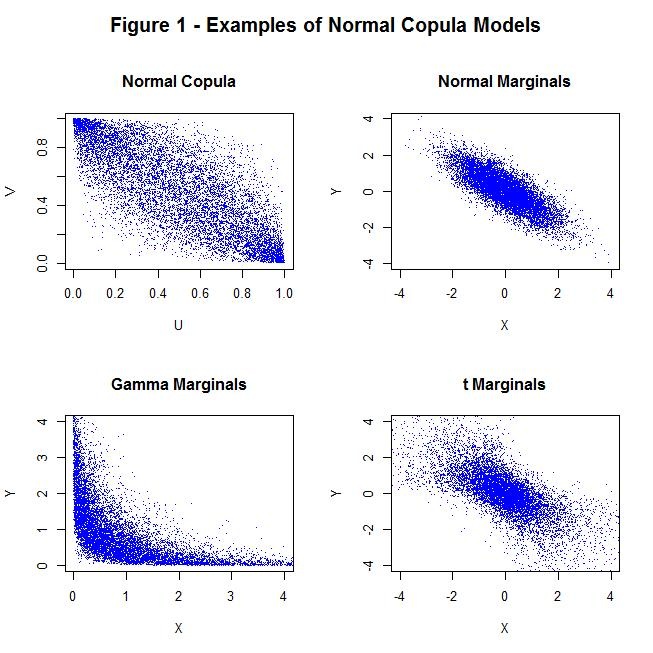
\includegraphics[width=0.9\textwidth]{copulas}
\end{figure}

\trish{Again impenetrable.  Expand and rewrite around an example:} The
forward implication of Sklar's theorem means that every distribution
can be rewritten in terms of a copula and univariate marginals. This
suggests that copulas encode the dependency structure stripped from
all the univariate marginal information like scale, shape and
location. If a copula can be obtained, then the corresponding
association structure can be studied via a \trish{copula density
function?}. The importance of the forward implication can also be seen
in \trish{Figure~\ref{fig:copula}}, where three obviously different
bivariate distributions, which are similar only with respect to a
general negative association between random variables $X$ and $Y$,
turn out to have identical association structure.
    
From \trish{delete: the} Sklar's theorem \trish{follow two} useful
corollaries \trish{delete: follow} that shed more light on how copulas
are useful in constructing new multivariate distribution
\citep{Joe1997,Nel2007}. The first corollary is an alternative
representation of a multivariate probability density function:
%
\newtheorem{cors}{Corollary}
\begin{cors}
\label{thm:density}
For a differentiable p--dimensional distribution function with
continuous quantile functions $F_1^{-1},
F_2^{-\trish{1}}, \dots, F_p^{-1}$, the probability density function
%
\begin{\trish{eqnarray*}}
\lefteqn{f(x_1,x_2, \dots, x_p)} &  =  &
       \frac{\partial^p F(x_1, x_2, \dots, x_p)}
             {\partial x_1 \partial x_2 \cdots \partial x_p} \nonumber \\ 
 & = & \frac{\partial^p C(F_1(x_1), F_2(x_2), \dots, F_p(x_p))}
             {\partial x_1 \partial x_2 \cdots \partial x_p} \nonumber \\
 & = & c(u_1, u_2, \dots, u_p)\prod_{i = 1}^p f(x_i).
\end{eqnarray*}
%
% 
\trish{Define the function $c$.}  The usefulness of
\trish{Corollary~\ref{thm:density}} is that it provides an alternative
way to construct a model by going directly to the probability density
function.

\trish{The results I have} presented so far provide an equation for
\trish{no: construction of new models}. However, any construction has
to be preceded by finding useful copulas \citep{Joe1997,Nel2007}. The
second corollary shows a simple way of obtaining a new copula:
%
\begin{cors}
\trish{\label{thm:copula}}
Let $F$ be a p-dimensional distribution function with continuous
quantile functions $F_1^{-1}, F_2^{-1}, \dots, F_p^{-1}$, then for
every $(u_1, u_2, \dots u_p) \in [0, 1]^p$
%
\begin{equation}
\label{eqn:copula}
C(u_1, u_2, \dots u_p) = F(F_1^{-1}(u_1), F_2^{-1}(u_2), \dots, F_p^{-1}(u_p))
\end{equation}
%
\end{cors}
%

\trish{Corollary~\ref{thm:copula}} implies that if one can specify an
existing multivariate distribution and derive its quantile functions,
then its copula is easily recoverable using
\trish{Equation~\ref{eqn:copula}}.  As a caveat, this method works
only if quantile functions can be obtained, which is \trish{not always
the case}. There are other methods for finding new copulas, and the
\trish{literature provides} a rich body of copulas to choose from
\citep{Joe1997,Nel2007}.

In conclusion, taking \trish{delete: the} Sklar's theorem and
\trish{its} two corollaries as a given, the problem of generalizing
the Ratcliff diffusion model to \trish{include} an association
structure \trish{among its parameters resolves to choosing} a copula
and univariate marginal distributions for each processing component
\citep{JohKot1994,JohKot1995}. Combining them using Sklar's
representation equation completes the construction. Thus, the
methodology of copulas provides a solution to the main problem of the
proposal.


%%%%%%%%%%%%%%%%%%%%%%%%%%%%%%%%%%%%%%%%%%%%%%%%%%%%%%%%%%%%%%%
\subsection{Predictive properties via Monte Carlo method}

\trish{This sentence is an example of passive voice: Once a
multivariate distribution with an association structure is specified a
new cognitive process model can be proposed.} \trish{Try to write in
active voice whenever possible: The proper selection of a multivariate
distribution with a covariance structure for the parameters permits us
to propose a new model.}  \trish{Note that the problem with the
previous sentence is that we aren't proposing a new model, so rewrite
it.}  \trish{We can now} explore the model's predictive \trish{and
estimation (explain)} properties, and \trish{evaluate} the model
against real performance data. I will use statistical methods to solve
all three problems.
	
\trish{delete:First,} Obtaining predictions from a generalized
diffusion model of simple decision making \trish{using fixed}
parameter values requires solving a triple integral of the mixture
model \citep{Tue2004}.  
%
\trish{Note: expand/rewrite this.  There's the mixture model arising
from the full Ratcliff model, and then there's your mixture using the
copula.  These statements don't say anything about the distinction
between the two, if indeed there is one, and it isn't clear whether
you're talking about something old or proposing something new: The
mixture density arises from integrating the Wiener first passage
density with respect to a mixing density, which encodes associations
between processing components via a copula. The complexity of the
equation makes the triple integral analytically intractable, so the
exact predictions cannot be obtained.}
%

Approximate predictions, however, can be calculated using the Monte
Carlo method \citep{RobCas2004,GamLop2006}. The application of the
Monte Carlo method \trish{sets} up an integration problem as
\trish{the} expected value of a function of a variable calculated
relative to \trish{an appropriate?} distribution. \trish{That is,
\[\text{put some math here using a } \approx \test{ symbol} and label
it \label{eqn:approx_sample}\].}  Using a \trish{large} sample
simulated from a distribution of interest and an appropriate law of
large numbers, an expected value can be estimated using the arithmetic
average of the function evaluated at each sampled draw.
	
\trish{Yuck.  Delete or rewrite, but I think you don't need this: The
mixture model of performance data fits with the Monte Carlo method
since it can be interpreted as an expected value of the Wiener first
passage density relative to a mixing density.}
% 
\trish{Note: Consistent with the hyper-thoroughness expected in a
thesis, and with the growing tendency of journal editors to demand a
public software repository for all routines used in a publication,
please expect to provide appendices of all your programs.  For the
thesis, these should include reasonably-informative commenting.}
%
Applying the \trish{Monte Carlo} method to obtain approximate
predictions requires solving three problems: sampling from a copula,
transforming each dimension according to a marginal quantile function,
and sampling from the Wiener first passage density. The first two
problems can be solved with the open-source R programming environment
that provides the package ``Copula'' to sample from a wide range of
copulas and the R base package that contains routines for marginal
quantile functions \citep{Rte2012,HofKoj2013}. I \trish{have
programmed a} sampler for the Wiener \trish{define: FPD} based on the
random walk approximation \citep[\trish{see
Appendix~\ref{app:sampler}]{TueMar2001}. All three pieces of software
can be conveniently and flexibly combined in an R program to obtain
approximate predictions for the proposed models.

%%%%%%%%%%%%%%%%%%%%%%%%%%%%%%%%%%%%%%%%%%%%%%%%%%%%%%%%%%%%%%%%%
\subsection{Bayesian inference via hierarchical models}

The problems of testing proposed models against real performance data
and establishing their estimation properties are methodologically
tied. Bayesian statistical theory provides a powerful and general
framework for solving both problems \citep{Ber1997,GelCar2013}. Recent
technological developments made the Bayesian approach ripe for
scientific use, and it is becoming popular in psychology, too
\citep{EdwLin1963,MyuPit1997,MyuKar2008,PerVan2002,RouLu2005,RouLu22005,CraPer2010,VanTue2011}. The
reasons for its appeal include representation of uncertainty with
probability, \trish{weird: coherent manipulation} of uncertainty using
probability calculus and ability to handle realistic models. I will
\trish{therefore conduct my research within} the Bayesian framework to
solve the derivative problems of model estimation and evaluation.

Unlike the \trish{still undefined: frequentist framework}, in the
Bayesian framework model parameters are treated as random variables
along with data. The full probability model, also called the Bayesian
model, is at the center of analysis
\citep{GelCar2013}. \trish{Ambiguous: It} requires specifying
\trish{the probability densities of both} data and
parameters. \trish{Ambiguous: These two building blocks} are assumed
to be conditionally dependent in a way that the full joint density can
be factored into a probability density of data given parameters,
called the likelihood, and the probability density of parameters,
called the prior. \trish{Note: your use of $X$ and $x$ is
inconsistent.  You need to say somewhere that $X=x$.}  Given a data
vector $\boldsymbol{X}\trish{={\bf{x}} \in \mathbb{R}^p$ and
\trish{data don't have parameters, and data are always plural: its}
parameter vector $\boldsymbol{\theta} \in \Theta \subseteq
\mathbb{R}^m$, a Bayesian model \trish{is written as} 
%
\begin{equation} f(\boldsymbol{x}, \boldsymbol{\theta}) =
      f(\boldsymbol{x} \mid \boldsymbol{\theta})f(\boldsymbol{\theta}) 
\end{equation} 
%
where $f(\boldsymbol{x} \mid \boldsymbol{\theta})$ is the likelihood
function and $f(\boldsymbol{\theta})$ is the prior \trish{density for
$\theta$}. The \trish{ability to factor the joint density of
${\bf{x}}$ and ${\bf{\theta}}$ into the likelihood and the prior} is
useful for constructing new Bayesian models because it allows breaking
the problem into manageable pieces, often consisting of common
univariate distributions \citep{JohKot1994,JohKot1995}.

\trish{For my thesis,} I will fit and test generalized cognitive
process models by incorporating them into hierarchical Bayesian models
\citep{Ber1997,GelCar2013}. This choice \trish{of what?} is motivated
by the structure of performance data. A typical experiment generates
multiple observations for each of several participants engaged in the
same task \citep{RatMck2008,Wag2009}. When specifying a statistical
model, the \trish{experimenter must choose whether to} treat
individual observations as coming from different sources or the same
source \citep{RouLu2005,RouLu22005,RouMor2014}. \trish{Need more here:
what does data pooling have to do with this choice?} Not pooling the
data presupposes no relation between the individuals while completely
pooling data ignores individual differences. However, for human
performance data, it is more accurate to assume a middle ground. Real
data varies among participants, but due to similarity in cognitive
abilities and experimental treatment, participants share
regularities. A hierarchical statistical model acknowledges this mixed
structure by assuming that individual parameters are a random sample
from a population, and introduces \trish{are you making up words?
semi-pooling} by fitting all the data simultaneously.
    
In a hierarchical model, the parameter space can be factored
\trish{delete: out} into parameters representing the individuals and
hyperparameters representing a population from which the
\trish{individuals' parameters} are sampled. \trish{(Need and $X=x$
here, as above.)}  With data $\boldsymbol{X} \in \mathbb{R}^p$
conditionally dependent on parameters $\boldsymbol{\theta} \in \Theta
\subseteq \mathbb{R}^m$, and parameters conditionally dependent on
hyperparameters $\boldsymbol{\psi} \in \Psi \subseteq \mathbb{R}^n$, a
hierarchical model
%
\begin{equation}
f(\boldsymbol{x}, \boldsymbol{\theta}, \boldsymbol{\psi}) =
f(\boldsymbol{x} \mid \boldsymbol{\theta})
f(\boldsymbol{\theta} \mid \boldsymbol{\psi})
f(\boldsymbol{\psi})
\end{equation}
%

can be factored into the likelihood $f(\boldsymbol{x} \mid
\boldsymbol{\theta})$, \trish{the prior} density of \trish{the
individual-level} parameters $f(\boldsymbol{\theta} \mid
\boldsymbol{\psi})$ and \trish{the prior} density of \trish{the}
hyperparameters $f(\boldsymbol{\psi})$. Construction of a
\trish{delete: new} Bayesian model \trish{is the selection of}
distributions for these three \trish{components of the joint
distribution}. I will construct hierarchical models to study
estimation properties of generalized diffusion models and test them
against \trish{define: benchmark data.}


%%%%%%%%%%%%%%%%%%%%%%%%%%%%%%%%%%%%%%%%%%%%%%%%%%%%%%%%%%%%%%%%
\subsection{Blocked DE-MCMC sampler}


\trish{After} a Bayesian model has been specified, inference about
unknown parameters can proceed by applying \trish{the} calculus of
probabilities. In the Bayesian framework, parameter estimation is
formalized as an instance of \trish{here and elsewhere: Bayes'}
theorem 
% 
\begin{equation} 
\trish{\label{eqn:posterior}}
\pi(\boldsymbol{\theta} \mid \boldsymbol{x}) = 
   \frac{f(\boldsymbol{x} \mid \boldsymbol{\theta}) \pi(\boldsymbol{\theta})} 
        {\idotsint\limits_\Theta f(\boldsymbol{x} \mid \boldsymbol{\theta})
         \pi(\boldsymbol{\theta})d\boldsymbol{\theta}}, 
\end{equation} 
% 
where $f(\boldsymbol{x} \mid \boldsymbol{\theta})$ is the likelihood
function, $\pi(\boldsymbol{\theta})$ is the prior distribution and
$\pi(\boldsymbol{\theta} \mid \boldsymbol{x})$ is the posterior
distribution \citep{Ber1997,CasBer2002,GelCar2013}. \trish{Delete:
The} Bayes' theorem implies that the posterior distribution is a
compromise between the likelihood and the prior. \trish{After} the
posterior is \trish{obtained,} various statistical \trish{procedures},
such as \trish{calculation of point and interval} estimates,
hypothesis tests and model checks, can be \trish{performed}.

In practice, application of \trish{delete: the} Bayes' theorem is
complicated by the integral in the denominator \trish{of
Equation~\ref{eqn:posterior}}. \trish{Relate to the numerator, what is
the FPT pdf in the equation?: For instance, the first passage time
density of the two-boundary Wiener process is intractable, so the
posterior density cannot be calculated exactly.}  \trish{However, we
can obtain} an approximation \trish{to the posterior} by applying a
special class of Monte Carlo algorithms that use Markov chains (MCMC)
to sample from the posterior density
\citep{RobCas2004,GamLop2006,GivHoe2012,GelCar2013}. \trish{Delete:
The} Inference calculations can be rewritten as expected value
problems, so a sample from the posterior density can be used to obtain
\trish{this part of the sentence is nonsensical: approximate answers
to what?, including the? Do you mean even using such?  complicated
models} \trish{as} the hierarchical diffusion model
\citep{PerVan2002,CraPer2010,VanTue2011}.

\trish{Note: Because you haven't yet defined a sampler, the following
paragraph assumes that the reader knows already what you're talking
about.  Perhaps refer back to the original equation
Eqn.~\ref{eqn:approx_sample} and reorient the paragraph around that.}
% \trish{Delete: The aim of} MCMC methods \trish{delete: is to}
\trish{sample from} regions of high probability density \trish{of the
posterior} and \trish{doesn't work any more: explore them starting
from an arbitrary starting point.} Such stochastic search and
exploration is conducted by simulating a discrete time, continuous
state-space Markov chain \citep{KarTay1975,KarTay1981,Ros2014}. The
mathematical description of the exploration is a transition kernel of
a Markov chain, which is a conditional distribution function
describing where the chain is likely to be next given where it is
right now. MCMC \trish{define: samplers} define a special kind of
transition kernel that has a limiting distribution and is
time-reversible. \trish{Note: you need to relate a chain to a sample.}
The sampler is constructed in such a way that the target distribution
\trish{(the posterior)}, is equivalent to the limiting
distribution. \trish{This should start the paragraph: Thus, MCMC
algorithms provide a method for sampling from arbitrary distributions
for which a likelihood function can be specified.}
    
\trish{Note reordering: One way to understand how an MCMC algorithm
works is by examining its transition kernel, which consists of a
proposal density that can explore the whole target space, and an
acceptance probability function that enables visiting both high and
low probability density regions.  I will use blocked differential
evolution MCMC (DE-MCMC) to simulate from the posterior density
\citep{Ter2006,TurSed2013}. The DE-MCMC is a genetic algorithm that
uses a system of interrelated, multivariate Markov chains to explore
the parameter space.}
    
\trish{Note: this description is not detailed enough to provide
insight to a non-expert.}  \trish{After} the chains are initialized,
the DE-MCMC algorithm updates one chain at a time in a deterministic
order. The proposal density perturbs the current position
$\boldsymbol{\theta}_{k, i - 1}$ of the kth chain by adding
independent noise $\varepsilon$ and a weighted difference of states of
two other randomly picked chains $\upsilon(\boldsymbol{\theta}_{m, i -
1} - \boldsymbol{\theta}_{n, i - 1})$. The independent noise
$\varepsilon$ is a proposal mechanism akin to many other samplers,
such as Metropolis-Hastings, and requires tuning
\citep{RobCas2004,GamLop2006}. The novel piece is using distances
between states of other chains, weighted by a positive scalar, to
update the current chain. The weight $\upsilon$ is the second tuning
parameter.
    
%\vspace{5mm}
%

\trish{Don't do it this way.  Use the "algorithm" package.  Figure
captions go underneath, not above.  Use the "figure" environment and
\label{fig:de-mcmc}.}

\centerline{\textbf{Figure 2 - Global DE-MCMC}}

\fbox{
\parbox{\textwidth}{
\begin{enumerate}
\item $\forall k \in \{1, 2, \dots, K\}$, initialize $\boldsymbol{\theta}_{k, 1} \ni \pi(\boldsymbol{\theta}_{k, 1} \mid \boldsymbol{x}) > 0$
\item for $i^{th}$ iteration in $2, 3, \dots, I$
\item \quad for $k^{th}$ chain in $1, 2, \dots, K$
\item \qquad Sample $\boldsymbol{\theta}_{m, i-1}, \boldsymbol{\theta}_{n, i-1}$ without replacement from \\ 
$\{\boldsymbol{\theta}_{1, i-1}, \boldsymbol{\theta}_{2, i-1}, \dots, \boldsymbol{\theta}_{K, i-1}\} \backslash \{\boldsymbol{\theta}_{k, i-1}\}$
\item \qquad Sample $\upsilon \sim \mathcal{U}(0.5, 1)$
\item \qquad Sample $\varepsilon \sim \mathcal{U}(-0.001, 0.001)$
\item \qquad Propose $\boldsymbol{\theta}^* = \boldsymbol{\theta}_{k, i-1} + \upsilon(\boldsymbol{\theta}_{m, i - 1} - \boldsymbol{\theta}_{n, i - 1}) + \varepsilon$
\item \qquad Sample $\alpha \sim \mathcal{U}(0, 1)$
\item \qquad if $\alpha < \frac{\pi(\boldsymbol{\theta}^* \mid \boldsymbol{x})}{\pi(\boldsymbol{\theta}_{k, i-1} \mid \boldsymbol{x})}$, then $\boldsymbol{\theta}_{k, i} = \boldsymbol{\theta}^*$
\item \qquad else $\boldsymbol{\theta}_{k, i} = \boldsymbol{\theta}_{k, i-1}$
\item \quad end for
\item end for
\end{enumerate}
	}
}

%\vspace{5mm}
%
%\noindent 

\trish{Note: Don't try to typeset the location of floating elements.
Let LaTeX make those decisions.}  \trish{Note: this paragraph is in
reverse order.  Reference the algorithm first, then go through it step
by step for the reader.}  The difference vectors \trish{$\theta_? -
\theta_?$} reflect the geometry of the high probability regions, where
most chains will reside if the algorithm is working, and improve
sampling. Given the proposed value $\boldsymbol{\theta}^*$,
\trish{define: the acceptance probability function} determines whether
the chain moves or stays. The DE-MCMC uses the same kind of acceptance
function as \trish{the} Metropolis-Hastings \trish{algorithm
\cite{refs}}. \trish{Figure~\ref{fig:de-mcmc}} gives an algorithmic
representation of such a transition kernel. The steps describe a
global DE-MCMC algorithm that moves chains through the whole parameter
space at once.

\trish{The blocked DE-MCMC algorithm is most appropriate for my
thesis} because it works well with highly correlated parameter spaces
\citep{TurSed2013}\trish{, such as the parameter space of the}
Ratcliff diffusion model \citep{RatTue2002}\trish{. Delete:, and is
likely to be inherited by the generalized models.} \trish{I don't
understand the rest of this paragraph: In addition, real data
problems, including applying generalized diffusion models to reaction
times and accuracy, involve high-dimensional parameter
spaces. \trish{This doesn't make sense.  Aren't we using a blocking
algorithm?  Rewrite: Without partitioning the parameter space into
blocks the computational efficiency of the algorithm is seriously
reduced.}}
 
\trish{Note: This paragraph does not accomplish what you want, because
you have not explained or defined anything. It needs to be greatly
expanded, and, indeed, probably deserves an entire subsection all on
its own.}
%
\trish{Segue missing.  Is partitioning the same as blocking?} A common
partitioning scheme, called Gibbs sampling, breaks apart the parameter
space into univariate blocks
\citep{RobCas2004,GamLop2006,GelCar2013}. However, \trish{because of}
correlations between parameters in cognitive process models, it will
be more efficient to work with blocks of several correlated
dimensions. Exploring the space in several dimensions simultaneously
will increase chances of proposing an acceptable move. Hence, the
best, if not always obvious, blocking scheme is to group correlated
parameters together and keep relatively independent parameters
separate. \trish{Figure~\ref{fig:blocked}} shows an example of a
blocked DE-MCMC for a hierarchical model of $J$ participants each
generating $N$ normal observations \trish{such that (note that all the
parameters below are undefined, so I have no idea what you're trying
to do here)}
%
\begin{gather}
\psi_{\mu} \sim \mathcal{N}(0, 10000), \quad 
\chi_{\mu} \sim \mathcal{G}(0.01,0.01)\trish{,} \nonumber \\
\psi_{\sigma^2} \sim \mathcal{G}(0.01, 0.01), 
\quad \chi_{\sigma^2} \sim \mathcal{G}(0.01,0.01)\trish{,} \nonumber \\
\mu_j \sim \mathcal{N}(\psi_{\mu}, \chi_{\mu}), 
\quad \sigma_j^2 \sim \mathcal{TN}(\psi_{\sigma^2}, \chi_{\sigma^2})\trish{, and} \nonumber \\
X_{n, j} \sim \mathcal{N}(\mu_j, \sigma_j^2)\trish{.} \nonumber
\end{gather}
%
\trish{What example? You need to explain what you're doing: In this
example,} the blocked DE-MCMC explores the model's parameter space by
updating one pair of means and variances at a time.

As any other MCMC algorithm, the DE-MCMC will generate a sample from
the posterior that is autocorrelated and is only guaranteed to
converge to the target distribution asymptotically
\citep{RobCas2004,GamLop2006}. To ensure the quality of samples,
before calculating any inferences, I will use graphical and numerical
methods to diagnose convergence of chains to the target density. These
methods are heuristics that do not guarantee convergence, but their
failure guarantees failure of convergence.
    
The standard graphical tools will include trace plots to examine the
time series of samples, and autocorrelation plots to gauge mixing of
the sampler, or how well the chains move around. I will use the trace
plot by overlaying many chains and observing if they stabilize around
the same point, which is strong evidence for convergence. Also, the
trace plot will help to determine the burn-in period, the initial
iterations that take the algorithm to find the high density region
from an initial state. In contrast, the autocorrelation plot will
assist in checking the proposal tuning, and whether the blocking
scheme combines highly correlated parameters. High autocorrelation
would indicate issues with either/both of these design choices.

%\vspace{5mm}

\trish{See comments on Figure 2 above.}
\trish{\label{fig:de-mcmc-blocked}}

\centerline{\textbf{Figure 3 - Blocked DE-MCMC}}
\fbox{
\parbox{\textwidth}{
\begin{enumerate}
\item $\forall k \in \{1, 2, \dots, K\}$, initialize $\boldsymbol{\theta}_{k, 1} \ni \pi(\boldsymbol{\theta}_{k, 1} \mid \boldsymbol{x}) > 0$
\item for $i^{th}$ iteration in $2, \dots, I$
\item \quad for $k^{th}$ chain in $1, \dots, K$ use the DE-MCMC kernel to sample
\item \qquad $(\psi_{\mu}, \chi_{\mu})^i \mid (\mu_1, \sigma_1^2, \mu_2, \sigma_2^2, \dots, \mu_J, \sigma_J^2)^{i-1}$
\item \qquad $(\psi_{\sigma^2}, \chi_{\sigma^2})^i \mid (\mu_1, \sigma_1^2, \mu_2, \sigma_2^2, \dots, \mu_J, \sigma_J^2)^{i-1}$
\item \qquad for $j^{th}$ participant in $1, 2, \dots, J sample$
\item \quad \qquad$ (\mu_j, \sigma_j^2) \mid (\psi_{\mu}, \chi_{\mu}, \psi_{\sigma^2}, \chi_{\sigma^2})^{i-1}$
\item \qquad end for
\item \quad end for
\item end for
\end{enumerate}
	}
}

%\vspace{5mm}
	
\trish{(Note parallel construction:) The numerical tools will include}
the \citet{GelRub1992} convergence statistic \trish{and} the potential
reduction scale factor (PRSF), that detects stationarity of chains by
comparing between-chain to within-chain variance
\citep{BroGel1998}. \trish{What are you doing here?  Explain.  Why
aren't you going into this kind of detail for the Gelman-Rubin
statistic?} For $i = 1, 2, \dots, m$ chains, let $\theta_{i, j}$ be
$j^{th}$ of $n$ iterations of a univariate parameter $\theta$ with
mean $\mu$ and variance $\sigma^2$, then the between-chain variance
%    
\begin{equation}
B = \frac{n}{m(n-1)}\sum_{i=1}^m(\theta_i - \overline\theta)^2
\end{equation}
and the within-chain variance
%
\begin{equation}
W = \frac{1}{m(n-1)}\sum_{i=1}^m \sum_{j=1}^n(\theta_{i,j} - \overline\theta_j)^2 = \frac{1}{m}\sum_{i=1}^m s_i^2
\end{equation}
%
are combined to calculate the pooled posterior variance estimate 
%
\begin{equation}
\hat V = \frac{n}{n-1}W + (\frac{1}{mn} + \frac{1}{n})B\trish{.}
\end{equation}
%
Then a corrected PRSF
%
\begin{equation}
\hat R = (\frac{d+3}{d+1})\frac{\hat V}{W}
\end{equation}
%
with \trish{delete: the} degrees of freedom
%
\begin{equation}
d \approx \frac{2 \hat V^2}
{\operatorname{\hat {var}} (\hat V)}
\end{equation}
%
and the variance estimate
%
\begin{eqnarray}
\operatorname{\hat {var}}(\hat V) & = & (\frac{n-1}{n})^2 \frac{1}{m} \operatorname{\hat {var}}(s_j^2) + \frac{m+1}{mn}^2 \frac{2}{m-1}B^2 + \nonumber \\
& + & 2\frac{(m+1)(n-1)}{m^2n}(\operatorname{\hat {cov}}(s_j^2,\overline\theta_j) - 2\overline\theta\operatorname{\hat {cov}}(s_j^2,\overline\theta))
\end{eqnarray}
%
\trish{...? this is not a grammatical sentence.}
\trish{What does this mean? I will treat a posterior sample with $1 \leq \hat R \leq 1.05$.}

%%%%%%%%%%%%%%%%%%%%%%%%%%%%%%%%%%%%%%%%%%%%%%%%%%%%%%%%%%%%%%%%
\subsection{Model selection via \trish{the} Bayesian predictive information criterion}

Model selection, a kind of statistical inference, arises when several
competing models are proposed to describe the same data.
\trish{Selection} criteria can be \trish{either} qualitative \trish{or
quantitative}
 \citep{MyuKar2008,ShiLee2008,VanMat2014}. 

In psychology, interpretability of the parameters and \trish{the}
plausibility of explanation it provides for data are important
qualitative criteria. The generalized diffusion models I intend to
propose will inherit the simple decision making interpretation for
\trish{define - what is an association vs. a non-association
parameter?:} non-association parameters, and the association
parameters may be interpreted as processing coordination imposed by
cognitive control processes. \trish{Why not?  This is probably the
biggest weakness in your proposal, that you have not considered
mechanisms for association across trials.  There are lots of theories
in the literature that you could use to justify such associations, and
you can think up some interesting ones yourself.  Then the project
becomes confirmatory rather than exploratory, and much much nicer and
more important as a result.  See the third item on the to-do list: The
explanatory plausibility cannot be judged a priori, and will be
determined by applying the models to real performance data.}
    
In contrast to qualitative considerations, a common quantitative
approach to model selection is based on model generalizability
\citep{GelHwa2013}. Generalizability is defined as model's
\trish{ability to predict} out-of-sample data collected under the same
conditions. A model with better generalizability \trish{can be
considered} a better approximation of the \trish{actual
data-generating mechanism}. One way to interpret \trish{what? this}
from the Bayesian perspective is to consider the posterior predictive
distribution
%
\begin{equation}
f(\boldsymbol{y} \mid \boldsymbol{x}) = \int\limits_{\Theta} f(\boldsymbol{y} \mid \theta)\pi(\boldsymbol{\theta} \mid \boldsymbol{x})d\boldsymbol{\theta} = \operatorname{E_{\boldsymbol{\theta} \mid \boldsymbol{x}}}[f(\boldsymbol{y} \mid \boldsymbol{\theta}],
\end{equation}
%
where $\boldsymbol{y} \in \mathcal{R}^p$ is future data,
$\boldsymbol{x} \in \mathcal{R}^p$ is \trish{the} observed data and
$\boldsymbol{\theta} \in \Theta^n \subseteq \mathcal{R}^m$ is
\trish{the vector of parameters}. The posterior predictive
distribution \trish{strange, reword or delete sentence: encodes all
the predictions of an updated Bayesian model}. A generalizability
criterion should support selection of a model with the most accurate
posterior predictive distribution.

The various proposals for \trish{calculating} out-of-sample predictive
accuracy can be decomposed into two parts: an estimate of predictive
accuracy based on observed data and a penalty term. The penalty term
is a correction for overfitting \trish{from using} the same data both
for parameter estimation and model evaluation. \trish{Note: you just
said that the penalty term was something different from this.  Rewrite
to resolve the apparent contradiction: The overfitting of a model to
data is driven by model complexity, so the penalty term quantifies
model complexity.} A popular and easy-to-calculate generalizability
measure is deviance information criterion (DIC) \citep{SpiBes2002} \trish{given by \[DIC =...\]}
\trish{where}
%
\begin{equation}
\overline D = \operatorname{E_{\boldsymbol{\theta} \mid \boldsymbol{x}}}[-2\operatorname{log}f(\boldsymbol{x} \mid \boldsymbol{\theta})]
\end{equation}
%
\trish{is a measure of fit} and 
%
\begin{equation}
p_D = \operatorname{E_{\boldsymbol{\theta} \mid \boldsymbol{x}}}[-2\operatorname{log}f(\boldsymbol{x} \mid \boldsymbol{\theta})] + 2\operatorname{log}f(\boldsymbol{x} \mid \operatorname{E_{\boldsymbol{\theta} \mid \boldsymbol{x}}}[\boldsymbol{\theta}] + c
\end{equation}
%
\trish{is a penalty term.}  \trish{The DIC} was developed \trish{for}
hierarchical Bayesian models where complexity is quantified with
effective number of parameters $p_D$. The issue with DIC is that it
tends to pick overfitted models \citep{GelHwa2013}.  \trish{The}
Bayesian predictive information criterion 
% 
\begin{equation} BPIC = \overline D + 2p_D \end{equation} 
% 
was developed by \citet{Ano2007,Ano2011}, to correct bias in
\trish{the} DIC, which turns out to be equivalent to doubling the
penalty term. For a posterior sample obtained by an MCMC algorithm,
BPIC can be easily estimated with
%
\begin{equation}
\hat{BPIC} = -\frac{6}{N}\sum_{i=1}^N \operatorname{log}f(\boldsymbol{x} \mid \boldsymbol{\theta_i}) + 4\operatorname{log}f(\boldsymbol{x} \mid  \boldsymbol{\overline\theta})\trish{.}
\end{equation}
 
There are two conditions under which BPIC is applicable to
hierarchical Bayesian models \citep{Ano2011}. First, the derivation
assumes that the likelihood model does not include the exact
generating distribution, but is not far from the true model. The
second condition is \trish{that the} marginal posterior distributions
are unimodal and not too skewed. The empirical success of the Ratcliff
diffusion model \citep{RatMck2008,Wag2009,VanTue2011} and prior
hierarchical fits of the model suggest that both of these conditions
hold. Therefore, I will use BPIC for model selection when fitting
proposed models to \trish{benchmark data?}.

%%%%%%%%%%%%%%%%%%%%%%%%%%%%%%%%%%%%%%%%%%%%%%%%%%%%%%%%%%%%%
\subsection{Model checking using posterior predictive checks}

Model selection based on predictive accuracy is useful for ordering a
set of competing models and selecting the one that will make the best
predictions for future observations generated by the same
process. \trish{Delete: The output is a best model relative to the
competitors.} However, because selection criteria are scalar
quantities, they do not reveal which features of \trish{the} data the
best model predicts well and which feature it misses. That is, it does
not give a sense of absolute fit of a model to data. It is possible
that a model may be best in a set of alternatives, but miss all the
important features of \trish{the} data. Thus, in addition to model
selection, it is important to directly check a model against data. A
Bayesian approach to \trish{checking} the absolute fit and misfit of a
model is to compare its posterior predictive distribution to
\trish{the observed data.}

The comparison between observations and posterior predictive
distribution is formalized in the method of posterior predictive
checks \citep{GelGoe2000,GelCar2013}. \trish{Delete: I will
concentrate on the graphical method rather than numerical.} The
\trish{graphical} procedure requires selecting a pivotal, discrepancy
statistic $S(\:)$ that captures some interesting data feature. For
example, one may consider the quantile set $\{0.1, 0.3, 0.5, 0.7,
0.9\}$ for both correct and error response times as important features
that a model should capture. Then, a discrepancy statistic
$S(\boldsymbol{x}_{obs})$ is calculated for the observed data. The
model's predictions for the statistic \trish{delete: have to} reflect
uncertainty in the parameter, so a sample \trish{of, say, 250
observations} is taken randomly from the estimated posterior. For each
parameter value a data set is generated of the same size as the
observed data \trish{set}, and the discrepancy statistics
$S(\boldsymbol{y}_{rep,1}), S(\boldsymbol{y}_{rep,2}), \dots,
S(\boldsymbol{y}_{rep,250})$ are calculated. Then, one can plot the
$S(\boldsymbol{x}_{obs})$ against the posterior predicted distribution
of the statistic. The location of the observed value relative to the
high density region will reveal consistency between the model and
observations.
    
For performance data\trish{, I will} overlay the observed versus
predicted quantile-probability function to determine how well the
proposed models of simple decision making capture the joint behavior
of reaction times and responses. I will use the posterior predictive
checks to test adequacy of proposed models with respect to central
features of \trish{benchmark data?}.


%%%%%%%%%%%%%%%%%%%%%%%%%%%%%%%%%%%%%%%%%%%%%%%%%%%%%%%%%%%%%%%
\section{Proposed models}

\trish{Segue here}

\subsection{Models of across-trial variability}

\trish{Rewrite:} The main problem addressed by this thesis is
development of cognitive process models \trish{models don't do this,
techniques of analysis do: capable of recovering an association
structure between processing components} from response times and
response proportion data. I propose two new diffusion models that
could in principle \trish{no: solve this problem.}

Both models take the Wiener process as a description of the decision
process involved in simple decision making, but they differ in the
mixing densities that describe across-trial variability. I will work
with \trish{remind the reader what this is: bias parameterization},
and \trish{I don't understand what you're saying here: the starting
point can always be recovered from posterior samples of bias.} The
mixing densities \trish{of what?} describe variation and covariation
in the processing components \trish{this sentence is backwards:
including drift rate, bias and non-decision time.} \trish{Explain:
Construction of a new mixing density amounts to specifying a new
multivariate density.} Using Sklar's theorem the problem of
constructing a new multivariate density can be broken down to
selecting a copula and marginal probability density functions.
    
In proposing \trish{which? the two mixing densities} I aimed to choose
both flexible copulas and marginals. \trish{I don't see a Second:
First,} the copulas have to be flexible to encode different types of
association structures. Within the set of existing copulas, many
copulas, regardless of the dimension, are governed by a single
parameter that induces a particular kind of association
\citep{Joe1997,Nel2007}. For example, Archimedean copulas are
controlled by a single parameter and encode the same lower tail,
\trish{delete: or} upper tail, or all-positive associations for all
pairs of variables. However, since there is no prior information
available about the association structure between processing
components underlying simple decision making, it is sensible to start
modeling with more flexible copulas. I interpret flexibility as
\trish{the ability of the copula to produce} different associations
for each pair ranging from full negative to full positive dependence.
    
\trish{Explain what makes a copula elliptical: The elliptical class of
copulas} satisfies the flexibility criterion. Specifically, I propose
using the normal and t copulas from the elliptical class to encode
association structure into the model of simple decision making. The
first proposed model has a normal copula
%
\trish{Variable of integration is undefined.  Please unpack this
expression piece by piece.  Your description is way too brief:}
%
\begin{eqnarray}
\lefteqn{C_1 (\boldsymbol{u} \mid \rho_{1,2},\rho_{1,3},\rho_{2,3})} \\
  & = & \Phi_3(\Phi^{-1}(u_1),
               \Phi^{-1}(u_2),
               \Phi^{-1}(u_3) \mid \boldsymbol{P}_1) \nonumber \\
  & = & \int_{-\infty}^{\Phi^{-1}(u_1)} \int_{-\infty}^{\Phi^{-1}(u_2)} 
        \int_{-\infty}^{\Phi^{-1}(u_3)} 
        \operatorname{det}(2\pi\boldsymbol{P}_1)^{-\frac{1}{2}}
        \operatorname{exp}(-\frac{1}{2}\boldsymbol{x}^T
                                       \boldsymbol{P}_1
                                       \boldsymbol{x})d\boldsymbol{x}\trish{,}
\end{eqnarray}
%
\trish{Note: $\exp$ is the same as $\operatorname{exp}$ for most common functions.}
%
where $\Phi_3(\:)$ is a three dimensional standard normal distribution
function and $\Phi^{-1}(\:)$ is the normal quantile function. Note
that it is derived using \trish{Corollary~\ref{thm:copula}}. The
copula is governed by association parameters $\rho_{i,j} \in [-1, 1]$
for $i, j = 1, 2, 3$ through a positive definite association matrix
%
\begin{equation}
\boldsymbol{P}_1 = \left[ \begin{array}{ccc}
1 & \rho_{1, 2} & \rho_{1, 3} \\
\rho_{1, 2} & 1 & \rho_{2, 3} \\
\rho_{1, 3} & \rho_{2, 3} & 1
\end{array}
\right].
\end{equation}
%

From Sklar's theorem, coupling the normal copula with the normal
marginals will \trish{Repeating from before, you haven't defined
copulas well enough for me to understand this: result in the
multivariate normal CDF}, but substituting some other marginals into
the normal copula will result in novel probability distributions.

Similarly, the second proposed model will have a \trsih{$t$} copula
\trish{given by}
%
\trish{See notes on the normal copula above.  Also flatten these expressions:}    
%
\begin{eqnarray}
\lefteqn{C_2(\boldsymbol{u} \mid \rho_{1,2},\rho_{1,3},\rho_{2,3},\omega)}
 & = & T_3(t^{-1}(u_1 \mid \omega),
           t^{-1}(u_2 \mid \omega),
           t^{-1}(u_3 \mid \omega) \mid \boldsymbol{P}_2) \nonumber \\ 
 & = & \int_{-\infty}^{t^{-1}(u_1 \mid \omega)}
       \int_{-\infty}^{t^{-1}(u_2 \mid \omega)}
       \int_{-\infty}^{t^{-1}(u_3 \mid \omega)}
       \frac{\Gamma(\frac{\omega+d}{2})}
            {\Gamma(\frac{\omega}{2})\sqrt{(\omega\pi)^d 
             \operatorname{det}(\boldsymbol{P}_2)}}
       \left( 1 + 
              \frac{\boldsymbol{x}^T\boldsymbol{P}_2^{-\frac{1}{2}}\boldsymbol{x}}
                   {\omega} \right),
\end{eqnarray}
%
where $T_3$ is a three dimensional \trish{$t$} cumulative distribution
function, $\Gamma(\:)$ is \trish{the} univariate gamma function and
$t^{-1}(\:)$ is a t quantile function. \trish{The} t copula is also
derived via corollary 2. The t copula is \trish{delete: similarly}
parameterized with an association matrix
%
\begin{equation}
\boldsymbol{P}_2 = \left[ \begin{array}{ccc}
1 & \rho_{1, 2} & \rho_{1, 3} \\
\rho_{1, 2} & 1 & \rho_{2, 3} \\
\rho_{1, 3} & \rho_{2, 3} & 1
\end{array}
\right],
\end{equation}
%
but also has a parameter $\omega > 0$ that influences \trish{the}
heaviness of the tails. The parameter \trish{$\omega$} introduces
\trish{delete: an} additional flexibility that controls probability of
extreme values in the tails and variable combinations \trish{of what}
that \trish{wrong word: contradict} the association structure. 

\trish{Break paragraph:} For example, if \trish{an} association
between two variables is positive, it is unlikely \trish{that we
might} observe a pair of values where one point has high magnitude and
the second point has low magnitude. \trish{However, the occurence} of
\trish{such} rare events is predicted for finite values of
\trish{$\omega$. As} \trish{$\omega$ tends to infinity,} the t copula
converges to the normal copula. Thus, the cognitive process model
based on the t copula is a further generalization of the normal copula
that allows modeling associations between processing components that
sometimes take unusual values \trish{delete: , that is break the
general coordination pattern.}

To complete the construction of the mixing densities, Sklar's theorem
dictates that one specifies the marginal distributions for each
variable component of processing. The choice of marginal distributions
is meant to preserve \trish{the} successful \trish{fits} of the
Ratcliff model \trish{to data}, \trish{fits that are} robust to
\trish{these} distribution assumptions \citet{Rat2013},
\trish{something is wrong here: but also \trish{these choices can
include?}  distributions that can take more flexible shapes relative
to a uniform variate.}  \trish{Why are you bringing up the uniform
here?  Explain.}

\trish{Rewrite: You know what you're doing but no one else does.
Justify your choices:} For the drift rate $\delta$, in line with the
Ratcliff model, I will \trish{assume} a normal distribution. I will
replace the continuous uniform assumption for the non-decision
parameter $t^{er}$ with a truncated normal distribution,
\trish{justify: which adds more flexibility to the shape}. \trish{So
you're using truncated normals?  This is too hard to understand: The
truncation on both the left and right side can be fixed using a list
of $23$ studies fitting the Ratcliff diffusion model
\citep{MatWag2009} - explain how}. \trish{Justify: I will take the
minimum and maximum values ($0.206$ and $0.942$) from the reported
studies as truncation points, $a < b$.}  Lastly, the bias parameter
$\beta$ will follow a beta distribution because of its flexibility in
shape. \trish{The} univariate marginals \trish{for the three
parameters} are \trish{therefore}
%
\trish{Don't forget equation punctustion!}
\begin{eqnarray}
\delta & \sim & \mathcal{N}(\nu, \eta)\trish{,} \nonumber \\
\beta & \sim & \mathcal{B}(\lambda, \gamma)\trish{, \text{ and }} \nonumber \\
t^{er} & \sim & \mathcal{TN}(\chi,\phi,a,b)\trish{.}
\end{eqnarray}
 
Applying Sklar's theorem to the specified copulas and marginals will
result in $i = 1, 2$ new mixing distributions of the form
%
\begin{equation}
F_i(\delta,\beta,t^{er}) = C_i(F_{\delta}(\delta),F_{\beta}(\beta),F_{t^{er}}(t^{er})),
\end{equation}
%
from which one can \trish{delete: easily} obtain mixing densities by a
mixed \trish{partial} derivative
%
\trish{Notation problem: variable names (e.g., $\delta$) and numerical
values (e.g., $\delta$ are the same.  Fix.}
%
\begin{equation}
\frac{\partial^3}{\partial\delta
                  \partial\beta
                  \partial t^{er}} F_i(\delta,\beta,t^{er}) 
   = c_i(F_{\delta}(\delta),
         F_{\beta}(\beta),
         F_{t^{er}}(t^{er}))
         f_{\delta}(\delta),f_{\beta}(\beta),f_{t^{er}}(t^{er})\trish{.}
\end{equation}
 
The copula density and marginal densities have \trish{known} analytic
expressions \trish{delete: that are readily available}
\citep{Nel2007,CasBer2002,JohKot1994,JohKot1995}.  Direct application
of the Sklar's theorem ensures that both models of parameter
variability are valid distributions. This completes \trish{delete:
construction} the \trish{generalization} of \trish{the Ratcliff
diffusion model.}
    
Testing the usefulness of proposed models will require combining the
new mixing densities with the Wiener first passage density into
mixture densities to predict how response times and responses are
jointly distributed. This is the topic of the first proposed study.

\trish{This is a great place to list and describe Studies A, B and C.
Expand the paragraph above.}

%%%%%%%%%%%%%%%%%%%%%%%%%%%%%%%%%%%%%%%%%%%%%%%%%%%%%%%%%%%%%%%%
\section{Proposed studies}

\trish{Something here}

\subsection{Study A\trish{: Predictive Properties}

\trish{Study A} will examine \trish{the} predictive properties of the
\trish{generalized model.}  The predictive properties are a pattern of
effects on the marginal and joint features of performance data
attributable to an association structure. The data features I will
examine are the probability density functions of the correct and error
response times, the $\{0.025, 0.1, 0.3, 0.5, 0.7, 0.9, 0.975\}$
quantile set of the correct and error response times, and \trish{the}
probabilities of \trish{each} response \trish{delete: one and
two}. The combination of these features allows graphical and
quantitative comparison of the two \trish{generalized} diffusion
models with association structure \trish{to} the \trish{standard}
independent diffusion model.


\trish{Note: affect=verb except among clinical psychologists,
effect=noun except in infrequent expressions such as "effect a
change."}

To \trish{determine} how an association structure \trish{affects}
chosen data features I will examine \trish{Very confusing.  Do you
mean, "a range of parameter values reflecting those reported in
published fits of the diffusion model?": a collection of parameter
combinations that reflect estimates recovered in reported studies} and
several association structures \trish{do these folks talk about
associations?: \citep{MatWag2009}}. The combinations of \trish{huh?
non-association parameters} will resemble a typical experimental study
where stimulus difficulty is manipulated on a \trish{trial-by-trial}
basis, and speed/accuracy instructions and decision bias are
manipulated \trish{over blocks of trials}. \trish{I will conduct
simulations over?} four stimulus difficulty levels spanning near
chance to near-ceiling performance, speed and accuracy emphases, and
bias/no-bias conditions \trish{for a total of X simulated experimental
conditions}. Conditions affecting perceptual and response execution
are assumed to be \trish{huh? constant}. Environmental factors affecting
variability in decision process components are assumed to induce
slower error response times relative to correct response times, faster
error response times or symmetric response times. \trish{Table~\ref{tab:non-assoc}}
contains non-association parameter values representing the proposed
conditions based on ranges and means from 23 studies fitting the
Ratcliff diffusion model \citep{MatWag2009}.
    
\begin{table}[H]
\trish{\label{tab:non-assoc}}
\centering
\caption{\textbf{Non-association parameters}}
\begin{tabular}{|l*{9}{|c}|r|}
\hline
Set & $\alpha$ & $\nu_1$ & $\nu_2$ & $\nu_3$ & $\nu_4$ & $\lambda$ & $\chi$ & $\eta$ & $\gamma$ & $\phi$ \\ \hline
1 & 0.10 & 0.00 & 0.10 & 0.20 & 0.40 & 0.50 & 0.250 & 0.12 & 0.05 & 0.05 \\ \hline
2 & 0.10 & 0.00 & 0.10 & 0.20 & 0.40 & 0.50 & 0.250 & 0.05 & 0.15 & 0.05 \\ \hline
3 & 0.10 & 0.00 & 0.10 & 0.20 & 0.40 & 0.50 & 0.250 & 0.01 & 0.01 & 0.05 \\ \hline
4 & 0.10 & -0.20 & -0.05 & 0.05 & 0.20 & 0.65 & 0.250 & 0.12 & 0.05 & 0.05 \\ \hline
5 & 0.10 & -0.20 & -0.05 & 0.05 & 0.20 & 0.65 & 0.250 & 0.05 & 0.15 & 0.05 \\ \hline
6 & 0.10 & -0.20 & -0.05 & 0.05 & 0.20 & 0.65 & 0.250 & 0.01 & 0.01 & 0.05 \\ \hline
7 & 0.20 & 0.00 & 0.05 & 0.10 & 0.20 & 0.50 & 0.250 & 0.12 & 0.05 & 0.05 \\ \hline
8 & 0.20 & 0.00 & 0.05 & 0.10 & 0.20 & 0.50 & 0.250 & 0.05 & 0.15 & 0.05 \\ \hline
9 & 0.20 & 0.00 & 0.05 & 0.10 & 0.20 & 0.50 & 0.250 & 0.01 & 0.01 & 0.05 \\ \hline
10 & 0.20 & -0.10 & -0.025 & 0.025 & 0.10 & 0.65 & 0.250 & 0.12 & 0.05 & 0.05 \\ \hline
11 & 0.20 & -0.10 & -0.025 & 0.025 & 0.10 & 0.65 & 0.250 & 0.05 & 0.15 & 0.05 \\ \hline
12 & 0.20 & -0.10 & -0.025 & 0.025 & 0.10 & 0.65 & 0.250 & 0.01 & 0.01 & 0.05 \\ \hline
\end{tabular}
\end{table}

\trish{For} each of the \trish{simulated} experimental conditions, I
will examine several association structures with low, medium and high
levels of association between processing components. The association
parameters for the normal and t copulas will be matched to ensure the
same level of association. Kendall's association coefficient, which
measures the amount of monotonic association between two variables,
suggests a way to match the two copulas. A convenient fact from copula
theory is that Kendall's coefficient \trish{huh? depends only on a copula}
\citep{Joe1997,Nel2007}. For elliptical copulas used in the proposed
models the Kendall's coefficient is
%
\begin{equation}
\psi = \frac{2}{\pi} \arcsin(\rho),
\end{equation} 
%
\trish{This is incomprehensible.  Expand and explain.}
where $\rho$ is an association parameter of either \trish{a} normal or t
copula. This expression implies that the proposed models with the same
association parameters will have the same level of associations and
differ only in the tail dependence.

\trish{Table~\ref{tab:assoc}} contains values for association
parameters for several types of association structures. The structures
reflect a few of many possible association patterns that could exist
under typical experimental conditions. The all-positive and
all-negative structures will allow establishing effects of association
magnitude, sign and their interaction on the performance data. The
mixed structure will also allow establishing effects of magnitude, but
under mixed signs.

\trish{Don't fight with LaTeX typesetting until the end.}
\begin{table}[H]
\label{tab:assoc}
\centering
\caption{\textbf{Association parameters}}
\begin{tabular}{|l|c|c|r|}
\hline
Set & $\rho_{\nu,\lambda}$ & $\rho_{\nu,\gamma}$ & $\rho_{\gamma,\lambda}$ \\ \hline
1 & 0.15 & 0.15 & 0.15 \\ \hline
2 & 0.50 & 0.50 & 0.50 \\ \hline
3 & 0.85 & 0.85 & 0.85 \\ \hline
4 & -0.15 & -0.15 & -0.15 \\ \hline
5 & -0.50 & -0.50 & -0.50 \\ \hline
6 & -0.85 & -0.85 & -0.85 \\ \hline
7 & -0.15 & -0.15 & 0.15 \\ \hline
8 & -0.50 & -0.50 & 0.50 \\ \hline
9 & -0.85 & -0.85 & 0.85 \\ \hline
\end{tabular}
\end{table}

Some preliminary calculations suggest that introduction of a mixing
density with dependent components will mostly affect the right tail of
the mixture density. Specifically, the probability of extremely slow
response times will decrease, and the thickness of the right tail will
decrease, depending on the pattern and strength of associations. For
instance, strong positive association among all processing
\trish{components} leads to decreases in the tail features for the
correct response times and to increases for the error response
times. \trish{Show these effects if you have them, otherwise delete:
The effects are manifest either in graphical representation of the
correct and error probability densities, or the ${0.7, 0.9, 0.975}$
quantile set. The effects persist, but are not identical across
several empirically consistent combinations of non-association
parameters.} This suggests that the proposed study exploring a rich
set of parameter combinations should provide an adequate understanding
of how addition of an association structure to the diffusion model
\trish{affects} predictions of the response time and response data.

%%%%%%%%%%%%%%%%%%%%%%%%%%%%%%%%%%%%%%%%%%%%%%%%%%%%%%%%%%%%%%%%

\trish{Note: Remember above to define what you mean by estimation
properties.  It might be better just to say "Parameter Estimation."}

\subsection{\trish{Study B: Estimation Properties}}

Study B will address the problem of parameter recovery of the proposed
models using Bayesian inference. Accurate estimation of parameters is
necessary to draw reliable inferences about cognition from
data. Analytical examination of \trish{estimation properties?} of the
proposed models is intractable, so I will use Monte Carlo simulation
\trish{for what, exactly?}
\citep{RobCas2004,GamLop2006,GelCar2013}. \trish{huh? The overall
constraints on how I specify dimensions of the study} are related to
applying the proposed models to the \trish{Note: after many references
to this, this is the first the reader knows of "Study C."  Study C
should be described before anything else: benchmark data in Study C}
\citep{RatRou1998}.

\trish{Note: Don't use presumed float numbers in float labels.  Use
something mnemonic and let LaTeX worry about the numbers.}

\trish{huh? The abstract structure} of the benchmark dataset is
equivalent to a few participants observed under a multifactorial
design, with a moderate number of observations per
cell. \trish{Table~\ref{tab:parameters} contains proposed parameters
that fall in the ranges of values that are recovered in real
experiments \citep{MatWag2009}.  I will assume a design with three
participants \trish{under trial-by-trial} manipulation of stimulus
quality, and \trish{between block} manipulation of speed/accuracy
instructions. For each participant, I will use association values
specified in \trish{Table~\ref{tab:assoc}} that span \trish{the range}
from low to high \trish{levels} of association. The degrees of freedom
for the \trish{$t$} copula will be \trish{You haven't given enough
information for anyone to be able to understand why this is so.  Work
on this above: 5 to ensure a scenario where extreme combinations of
processing components are likely.} For all the stimulus/instruction
combinations I will \trish{examine sample sizes for each subject
\trish{by condition?} of} 50, 150, and 500 observations
\trish{because} these values are common from developmental to
cognitive psychology \citep{Luc1986,Wag2009,RouLu2005}.
    

\begin{table}[H]
\label{tab:parameters}
\centering
\caption{\textbf{True parameters}}
\begin{tabular}{|l*{11}{|c}|r}
\hline
Subject & $\alpha$ & $\nu_1$ & $\nu_2$ & $\nu_3$ & $\nu_4$ & $\lambda$ & $\chi$ & $\eta$ & $\gamma$ & $\phi$ \\ \hline
  I & 0.10 & -0.20 & -0.05 & 0.05 & 0.20 & 0.55 & 0.225 & 0.10 & 0.15 & 0.05 \\ \hline
  I & 0.20 & -0.10 & -0.025 & 0.025 & 0.10 & 0.60 & 0.225 & 0.10 & 0.15 & 0.05 \\ \hline
 II & 0.08 & -0.25 & -0.10 & 0.10 & 0.25 & 0.50 & 0.250 & 0.12 & 0.20 & 0.08 \\ \hline
 II & 0.16 & -0.13 & -0.05 & 0.05 & 0.13 & 0.55 & 0.250 & 0.12 & 0.20 & 0.08 \\ \hline
III & 0.12 & -0.15 & -0.08 & 0.08 & 0.15 & 0.60 & 0.275 & 0.08 & 0.18 & 0.12 \\ \hline
III & 0.18 & -0.075 & -0.04 & 0.04 & 0.075 & 0.65 & 0.275 & 0.08 & 0.18 & 0.12 \\
\hline
\end{tabular}
\end{table}

\trish{I can't understand this paragraph at all.  Isn't the point of
using copulas to be able to model non-independent observations without
a lot of theoretical overhead?  What does the experimental design have
to do with this?  Rewrite: Sampling will be conducted under assumption
of independent observations, thus ignoring the trend and
autocorrelation present in real data
\citep{PerVan2002,CraPer2010}. However, the experimental design
somewhat alleviates the issue of sequential dependencies. Because
stimulus is manipulated on each trial, the analysis is done on groups
of trials pulled at different trial points, as opposed to the actually
observed sequence. Such extraction breaks the temporal structure and
amounts to a kind of thinning process (i.e. removing elements of a
point stochastic process according to a predefined rule
\citep{RobCas2004,GamLop2006,GelCar2013,Ros2014}. The dependencies are
reduced with the greater number of stimulus quality conditions. The
\trish{huh? benchmark data} has 66 stimulus quality/instruction
conditions, so the independence assumption seems to be a plausible
approximation that will generalize conclusions to fitting new
diffusion models to the benchmark data.}
    
I propose three hierarchical Bayesian models whose estimation
properties will be explored under \trish{the simulation conditions
specified where?}. Using the factorization property of Bayesian models
I will specify the likelihood, priors and hyperpriors in order. For
each participant, the data set will contain $n$ observations, equally
split between $j = 1, 2, \dots, 4$ stimulus levels and $k = 1, 2$
instruction conditions. The $i^{th}$ observation of response time and
response \trish{follows the distribution of} a two-boundary Wiener
first passage time \trish{with} probability density
%
\begin{equation}
f(t_{i,j,k}^{rt}, r_{i,j,k} \mid \alpha_k, \delta_{i,j,k}, \beta_{i,j,k}, \tau_{i,j,k}^{er}),
\end{equation}

where processing parameters \trish{LIST} reflect \trish{the
assumptions} of \trish{the} effect of instructions on the threshold,
and across-trial variability. I will assume that each observation is
\trish{conditionally independent given} the processing parameters.

\trish{What was first? The second building block} is the prior. \trish{NO: The
proposed mixing densities act as priors in the Bayesian diffusion
model.}
%
\trish{Note: This may be a problem.  A mixture model is not the same thing
as a Bayesian model with priors equal to the mixing probabilities.  If
this is what you've assumed, then you need to realize that you are not
fitting the Ratcliff model in a Bayesian fashion, but rather a plain
vanilla, no parameter variability diffusion process model in a
Bayesian fashion.  The fact that I have just realized that you are
doing this (if in fact you are) indicates a pretty serious problem
with your exposition of the model.  Hopefully, all you need to do is
revise/delete this one sentence.}
%
Processing parameters undergo fluctuations from trial to trial
according to a copula-based density
%
\begin{eqnarray}
\lefteqn{f(\delta_{i,j,k},\beta_{i,j,k},\tau_{i,j,k}^{er} 
   \mid \nu_{i,j},\eta,\lambda_k,\gamma_k,\chi,\phi,\rho_{\tau^{er},\delta},
   \rho_{\beta,\delta},\rho_{\tau^{er},\beta})} \nonumber \\
  & = & c(F_{\delta}(\delta_{i,j,k}),F_{\beta}(\beta_{i,j,k}),F_{t^{er}}(\tau_{i,j,k}^{er}) 
        \mid \rho_{\tau^{er},\delta},\rho_{\beta,\delta},\rho_{\tau^{er},\beta}) \nonumber \\
  &   & \times f_{\delta}(\delta_{i,j,k} \mid \nu_{i,j}, \eta)
               f_{\beta}(\beta_{i,j,k} \mid \lambda_k,\gamma_k)
               f_{\tau^{er}}(\tau_{i,j,k}^{er} \mid \chi, \phi, 0.1, \operatorname{min}(\tau^{er})), 
\end{eqnarray} 
%
where $c(\:)$ defines a density for a copula, either an independent, a
normal or a t, and \trish{can incorporate one of} three different
association structures. The remaining marginal densities \trish{for
what} are \trish{the} normal, beta, truncated normal, respectively,
and are assumed to be the same for \trish{do you mean all the copulas?
all the models}. Finally, the prior specification is complete by
assuming the threshold parameter \trish{justify this:
%
\begin{equation} 
\alpha_k \sim \mathcal{U}(0.01, 0.45).  
\end{equation}
%}
\trish{See above.  You have not justified this well enough and it
conflicts with your previous presentation of the Ratcliff model:
Treating the association model as a prior fits neatly with the
Bayesian computation, where MCMC can be used to approximate the
posterior distribution and naturally implements the difficult integral
required to specify the mixture model of performance
data. \trish{Incomprehensible: Marginalizing over the trial specific
parameters is simply dropping nuisance parameters from analysis.}}
    
\trish{No first: The last building block} is the hyperprior density. I
will use informed priors based on long experience with the Ratcliff
diffusion model \citep{MatWag2009} for the non-association parameters,
but association parameters will be assigned diffuse priors to express
ignorance about this type of parameter. \trish{Expand and explain: The
full hyperprior density will differ for each model reflecting their
association structure.} The \trish{hyperparameters of the} independent copula diffusion model are
assigned \trish{hyperpriors such that}
%
\begin{gather}
\nu_{i,j} \sim \mathcal{U}(-1.00, 1.00)\trish{,} \nonumber \\
\eta \sim \mathcal{U}(0, 0.3)\trish{,} \nonumber \\
\lambda_k \sim \Gamma(2, 3), \nonumber \\
\gamma_k \sim \Gamma(2, 3), \nonumber \\
\chi \sim \mathcal{U}(0.10, 1.00), \test{ and} \nonumber \\
\quad \phi \sim \mathcal{U}(0, 0.35).
\end{gather}
%
The normal copula diffusion model adds the association parameters \trish{the} hyperpriors
\begin{eqnarray}
\rho_{\tau^{er},\delta} \sim \mathcal{U}(-1.00, 1.00), \nonumber \\
\rho_{\beta,\delta} \sim \mathcal{U}(-1.00, 1.00), \test{ and} \nonumber \\
\rho_{\tau^{er},\beta} \sim \mathcal{U}(-1.00, 1.00)
\end{eqnarray}

Finally, the \trish{$t$} copula diffusion model adds the \trish{you're
now calling this something new, and it was only a "flexibility"
parameter earlier.  Be consistent: degrees of freedom}
\trish{parameter $\omega$ with} hyperprior
%
\begin{equation}
\omega \sim \Gamma(1, 1)
\end{equation}
 
To establish \trish{the} statistical properties of the proposed
Bayesian models, each parameter-by-sample size combination will be
simulated 200 times to obtain a sampling distribution of posterior
means of all the unknown parameters, for the three proposed
models. \trish{So you're using frequentist methods to establish the
properties of a Bayesian posterior estimate?  How odd.  Justify why
you should do this.}  I will use root mean squared error
%
\begin{equation}
RMSE = \sqrt{\frac{1}{m}\sum_{i=1}^M (\theta^{true} - \operatorname{\hat E}_{\theta \mid x}[\theta]_i)^2}
\end{equation}
%
as a loss function to measure quality of hierarchical estimates
because it combines both bias and variability of an estimator
\citep{CasBer2002,RatTue2002,RouLu2005}. Successful application of the
proposed models will rely on obtaining accurate estimates with small
sample sizes and showing consistency of estimation as the sample size
grows. Both of these requirements can be checked under the proposed
simulation design by studying trends in RMSE.

%%%%%%%%%%%%%%%%%%%%%%%%%%%%%%%%%%%%%%%%%%%%%%%%%%%%%%%%%%
\subsection{\trish{Study C: Application to Benchmark Data}

\trish{Note: The details of the Ratcliff/Rouder study should be
provided much earlier in the proposal and used to orient the
discussion.}

The purpose of \trish{Study~C} is to evaluate the proposed models
against benchmark performance data. \citet{RatRou1998} ran a
brightness discrimination task with three participants \trish{delete:
(named NH, KR, and JF)}. On each trial, participants were asked to
decide whether a stimulus \trish{was of} ``high'' or ``low''
brightness \trish{according to what?}.  The stimulus was a pixelated
grid with $25\%$ \trish{of the pixels being} black and white
\trish{and shown as a center square}, and $75\%$ of \trish{the pixels
being} grey pixels \trish{and shown as} a frame around the square. The
proportion of white to black pixels was manipulated across
trials\trish{delete: by sampling stimuli from a discrete uniform
distribution with 33 equally spaced values}. Also,
\trish{between-block} instructions directed participants to
\trish{maximize} either speed or accuracy. Accuracy feedback was
presented after each trial, but \trish{the participants were provided
with no other information} about the \trish{ distribution of the
number of black/white pixels.}  \trish{Need detail here about how
accuracy was defined.}

The experiment lasted ten sessions and generated eight
\trish{102-trial} blocks of data for each session totaling 8160
observations per \trish{participant}. The \trish{say this differently:
interesting variables} include speed/accuracy instruction,
white-to-black pixel proportion, response times and responses. The
data \trish{demonstrate} phenomena, \trish{describe these: such as the
speed-accuracy trade off and the cross-over effect in mean response
times}, which are commonly used to test sequential sampling models
\citep{RatMck2008}. I will use this data set to test Bayesian versions
of three diffusion models of simple decision making.

\trish{Note: Everything from here on is legitimately a "Study C" that
can come after Studies A and B.}
    
Before specifying a Bayesian model, three features of performance data
need to be considered to motivate its construction. First, real data
is a mixture of responses, either produced by the processing
underlying simple decision making or by contaminant processes. Two
recognized types of contaminants are guesses and delayed responses
\citep{Rat1993,RatTue2002,VanTue2007,VanTue2008,
VanTue2011,CraPer2010}. These contaminant processes can arise from
non-compliance with experimental instructions or occasional loss of
attention\trish{, among other things}.
    
From \trish{an} analysis perspective, guesses do not involve any
stimulus encoding and evidence accumulation, so data generated by this
process \trish{carry} no information about the cognitive processing of
interest. Delayed responses, on the other hand, \trish{could} involve
belated stimulus processing and evidence accumulation, thus generating
data informative about the choice, but not the processing time.
    
\trish{Eliminate this from your proposal.  This is a very difficult
model to implement, and tangential to the goals of the proposal:} To
obtain accurate inferences about the process of interest from the
collected data, contaminants need to be either excluded or
modeled. Because exclusion rules (e.g. drop all data more extreme than
two and a half standard deviations away from the mean) are mostly
arbitrary, a more persuasive and informative approach is to explicitly
model contaminants. I will use a mixture model with latent class
assignment to deal with both guessing and delayed response.
    
The second important feature of the benchmark data set is the
proportion of black to white pixels covariate. Assuming selective
influence of stimulus quality on drift rate implies that with 33
stimulus conditions I will need to estimate 33 drift rates
\citep{VosRot2004}. A more parsimonious and revealing approach is to
regress the drift rate on the proportion
variable. \citet{VanTue2008,VanTue2011} successfully used the Weibull
psychometric function to connect drift rates to proportions of
pixels. I will incorporate the Weibull regression structure to
simplify my Bayesian models \citep{PerVan2002,Rat2014}.
    
The last notable feature of the brightness discrimination data is
sample sizes. The data \trish{consist of} a large number of individual
observations that should lead to well-informed inferences about
individual parameters using Bayesian updating. \trish{By} contrast,
having only three participants \trish{means that there can be} little
learning about group parameters \trish{delete: will occur together
with a significant increase in computational complexity}.  If a single
hierarchical Bayesian model is specified, assigning group priors can
add up to 26 dimensions to the parameter space. Given \trish{this
issue,} I will fit each participant's data separetely. \trish{Note
that not all model parameters need to be hierarchical.}

\trish{Eliminate contaminants:} The models I plan to evaluate are the
independent copula diffusion model with contaminants (DM1), the normal
copula diffusion model with contaminants (DM2) and the t copula
diffusion model with contaminants (DM3). Multiple variations of these
models could be constructed by making different assumptions about how
experimental manipulations influence cognitive processing. However, I
will rely on conclusions from studies analyzing the same data set to
constrain non-association parameters, and concentrate on examining the
association structure.

\trish{I skimmed the rest of this but made few comments.  You are
proposing to do too much, and I do not want you to tackle contaminant
components in this project.  Get the copula working, fix the problem
above with mixture vs. prior probabilities, simply fit that model to
the RatRou data, and then you'll be done.  You can worry about the
contaminants later.}

\trish{TRISH STOPPED HERE}
    
I will begin specifying models by describing a mixture likelihood
function of a single observation that could arise from a Wiener
process or contaminant processes. Assume that response ``high''
corresponds to the upper boundary and ``low'' to the lower
boundary. On each trial, a response time and response is generated by
a latent class of processes $C \in \{0, 1, 2\}$, representing a
decision process, a delayed decision process and a guessing process,
respectively. Then, under some stimulus level $j = 1, 2, \dots, 33$
and instruction condition $k = 1, 2$, the $i^{th}$ instance of
processing from 8160 trials belongs to a latent class $C_{i,j,k}$ with
unknown probability mass function
    
\begin{equation}
f(C_{i,j,k}) = 
\begin{cases}
p_{WD}, \quad C_{i,j,k} = 0 \\
p_{DD}, \quad C_{i,j,k} = 1 \\
p_{GD}, \quad C_{i,j,k} = 2
\end{cases}
\end{equation}
where ${p_{WD}}$ is the probability of Wiener decision, ${p_{DD}}$ is the probability of delayed decision and ${p_{GD}}$ is the probability of a guessed decision. For a given latent class $C_{i,j,k}$ and process parameters $\boldsymbol{\theta}_{C_{i,j,k}}$, the component joint densities of response time and response 

\begin{gather}
f(t_{i,j,k}^{rt},r_{i,j,k} \mid \boldsymbol{\theta}_{C_{i,j,k}}, C_{i,j,k}) = \nonumber \\
\begin{cases}
f_{WD}(t_{i,j,k}^{rt},r_{i,j,k} \mid \alpha_k,\delta_{i,j,k},\beta_{i,j,k},\tau_{i,j,k}^{er}, C_{i,j,k} = 0) \\
f_{DD}(t_{i,j,k}^{rt},r_{i,j,k} \mid \alpha_k,\delta_{i,j,k},\beta_{i,j,k},\operatorname{min}(t^{rt}),\operatorname{max}(t^{rt}), C_{i,j,k} = 1) \\
f_{GD}(t_{i,j,k}^{rt},r_{i,j,k} \mid \operatorname{min}(t^{rt}),\operatorname{max}(t^{rt}), C_{i,j,k} = 2)
\end{cases}
\end{gather}

	The Wiener decision component generates performance data according to the two-boundary first passage time probability density stated on page \pageref{eq:wd}. The delayed decision component is assumed to generate response times according to a continuous uniform density bounded by minimum and maximum observed response times, and responses as a Bernoulli random variable with probability parameter representing absorption of the Wiener process at the upper boundary. The delayed decision process joint density
\begin{gather}
f_{DD}(t_{i,j,k}^{rt},r_{i,j,k} \mid \theta_1, C_{i,j,k} = 1) = \nonumber \\ 
\frac{1}{\operatorname{max}(t^{rt}) - \operatorname{min}(t^{rt})}Pr(R_{i,j,k}=1)^{r_{i,j,k}}(1-Pr(R_{i,j,k}=1))^{1-r_{i,j,k}},
\end{gather}
where
\begin{equation*}
Pr(R_{i,j,k}=1) = \frac{\operatorname{exp}                   \{\frac{-2\delta_{i,j,k} \alpha_k \beta_{i,j,k}}{\sigma^2}
\} - 1}{\operatorname{exp}\{
\frac{-2\delta_{i,j,k} \alpha_k}{\sigma^2}
\} - 1}
\end{equation*}
Lastly, the guessed decision process is also assumed to generate response times according to a continuous uniform variate bounded by minimum and maximum observed response time. The response, however, is a Bernoulli random variable with probability parameter representing chance. The guessed decision process joint density
\begin{equation}
f_{GD}(t_{i,j,k}^{rt},r_{i,j,k} \mid \boldsymbol{\theta}_2, C_{i,j,k} = 2) = \frac{0.5}{\operatorname{max}(t^{rt})-\operatorname{min}(t^{rt})}
\end{equation}

	Usually, one would want to create a mixture distribution of processes by averaging out the latent class variable, but I will keep it as an unknown variable to be estimated from data. Building the latent class variable into the Bayesian model will enable not only to deal with contamination in a more principled way, but also to infer the proportion of contaminants in the data and latent membership of each observation \citep{LeeFus2007,LeeWag2014}.
    
	So far I have defined a probability density of a response time and a response for a single trial $i$ that depends on ordinal statistics and Wiener parameters. The ordinal statistics are estimated directly from the data, but the Wiener parameters require a prior. The prior decomposes into the latent class variable, which follows a categorical distribution stated above, and a model of unknown parameters. I will assign the three copula-based densities used in studies A and B as priors for the drift rate, bias and non-decision time. The general form of a copula-based prior has a probability density 
    
\begin{gather}
f(\delta_{i,j,k},\beta_{i,j,k},\tau_{i,j,k}^{er} \mid \nu_{i,j},\eta,\lambda_k,\gamma_k,\chi,\phi,\rho_{\tau^{er}},\rho_{\beta,\delta},\rho_{\tau^{er},\beta}) = \nonumber \\
c_{DM}\left(F_{\delta}(\delta_{i,j,k}),F_{\beta}(\beta_{i,j,k}),F_{\tau^{er}}(\tau_{i,j,k}^{er}) \mid \rho_{\tau^{er},\delta},\rho_{\beta,\delta},\rho_{\tau^{er},\beta}\right)
\times \nonumber \\
f_{\delta}(\delta_{i,j,k} \mid \nu_{i,j},\eta)f_{\beta}(\beta_{i,j,k} \mid \lambda_k, \gamma_k)f_{\tau^{er}}(\tau_{i,j,k}^{er} \mid \chi, \phi, 0.1, \operatorname{\tau^{er}}),
\end{gather}
where $c_{DM}(\:)$ is either an independent, a normal or a t copula, and marginal densities are normal, beta, truncated normal, respectively. Lastly, the threshold parameter prior density
\begin{equation}
\alpha_k \sim \mathcal{U}(0.01, 0.45).
\end{equation}

	The copula-based prior specifies a mean parameter drift rate for each stimulus level by instruction combination. This was not a burden in the estimation study with total of eight conditions, but 66 mean drift rates in the benchmark data unnecessarily complicate the model. A better solution is to incorporate the white-to-black proportion covariate through a regression function to describe how mean drift rate changes across experimental conditions. I assume the sigmoidal Weibull function of covariate   
\begin{equation}
\nu_{j,k} = \nu_k^{lo}+\left(\nu_k^{hi}-\nu_k^{lo}\right)   \left( 
1 - \operatorname{exp} 
\left( 
\frac{s_{j,k}}{\nu_k^{sc}} 
\right)
\right)^{\nu^{sh}},
\end{equation}

\noindent where $\nu^{lo}$ is the lower asymptote, $\nu^{up}$ is the upper asymptote, $\nu^{sc}$ is the scale parameter and $\nu^{sh}$ is the shape parameter. The parameter indices imply that the function changes in all its respects under speed/accuracy manipulation.

	The last structure needed to complete construction of hierarchical Bayesian models is the probability density of hyperparameters. The three competing models will vary in their hyperparameters. The distributional assumptions for DM1, the independent copula, are
    
\begin{gather}
\nu_k^{lo} \sim \mathcal{U}(-1.00, 0), \nu_k^{lo} \sim \mathcal{U}(0, 1.00) \nonumber \\
\nu_k^{sc} \sim \mathcal{U}(0, 1.00), \nu_k^{sc} \sim \mathcal{U}(0, 1.00) \nonumber \\
\eta \sim \mathcal{U}(0, 0.3) \nonumber \\
\lambda_k \sim \mathcal{G}(2, 3), \gamma_k \sim \mathcal{G}(2, 3) \nonumber \\
\chi \sim \mathcal{U}(0.10, 1.00), \phi \sim \mathcal{U}(0, 0.35) \nonumber \\
(p_{WD}, p_{GD}, p_{DD}) \sim \mathcal{D}(1, 1, 1) 
\end{gather}
For DM2 I add association parameters of the normal copula, the hyperprior 

\begin{eqnarray}
\rho_{\tau^{er},\delta} \sim \mathcal{U}(-1.00, 1.00) \nonumber \\
\rho_{\beta,\tau^{er}} \sim \mathcal{U}(-1.00, 1.00) \nonumber \\
\rho_{\beta,\delta} \sim \mathcal{U}(-1.00, 1.00) 
\end{eqnarray}
Lastly, the DM3 expands the DM2 by adding a degrees of freedom parameter to the hyperprior

\begin{equation}
\omega \sim \mathcal{G}(1, 1)
\end{equation}
For the non-association parameters, I rely on values collected from 23 studies fitting the Ratcliff diffusion model to assign informed priors using the minimum and maximum values \citep{MatWag2009}. Association parameters, latent class probabilities and degrees of freedom of a t copula are assigned diffuse priors to express current ignorance about them.

	The proposed Bayesian models can provide insights about coordination of cognitive processes by comparing several models of association structure. I will fit the three Bayesian models using the DE-MCMC and evaluate the predictive accuracy using BPIC. Comparison of BPIC values across models will provide evidence about the presence of associations under standard experimental manipulations. Finally, I will examine the central features of the data including response time distributions, accuracy rates under different stimulus conditions and the cross-over effect using posterior predictive checks to gauge the absolute fit of proposed models.


\bibliography{Slava_references}
\bibliographystyle{apa}

\end{document}